\documentclass[12pt,a4paper]{article}
\usepackage[utf8]{inputenc}
\usepackage[finnish]{babel}
\usepackage{setspace}
\usepackage{subcaption}
\usepackage{fancyhdr}
\usepackage{amssymb}
\usepackage{amsmath}
\usepackage{mathrsfs}
\usepackage[top=1in, bottom=1in, left=1in, right=1in]{geometry}
\usepackage{float}
\usepackage{pdfpages}
\usepackage{natbib}
\setcitestyle{semicolon}

\usepackage{titlesec}
\titleclass{\section}{top}
\newcommand\sectionbreak{\clearpage}
\titleformat*{\section}{\Huge\bfseries}
\titleformat*{\subsection}{\Large\bfseries}
\titleformat*{\subsubsection}{\large\bfseries}

\usepackage{hyperref}
\hypersetup{pdfborder={0 0 0}}
\onehalfspacing
\cfoot{}
\setlength{\parindent}{0pt}

\begin{document}

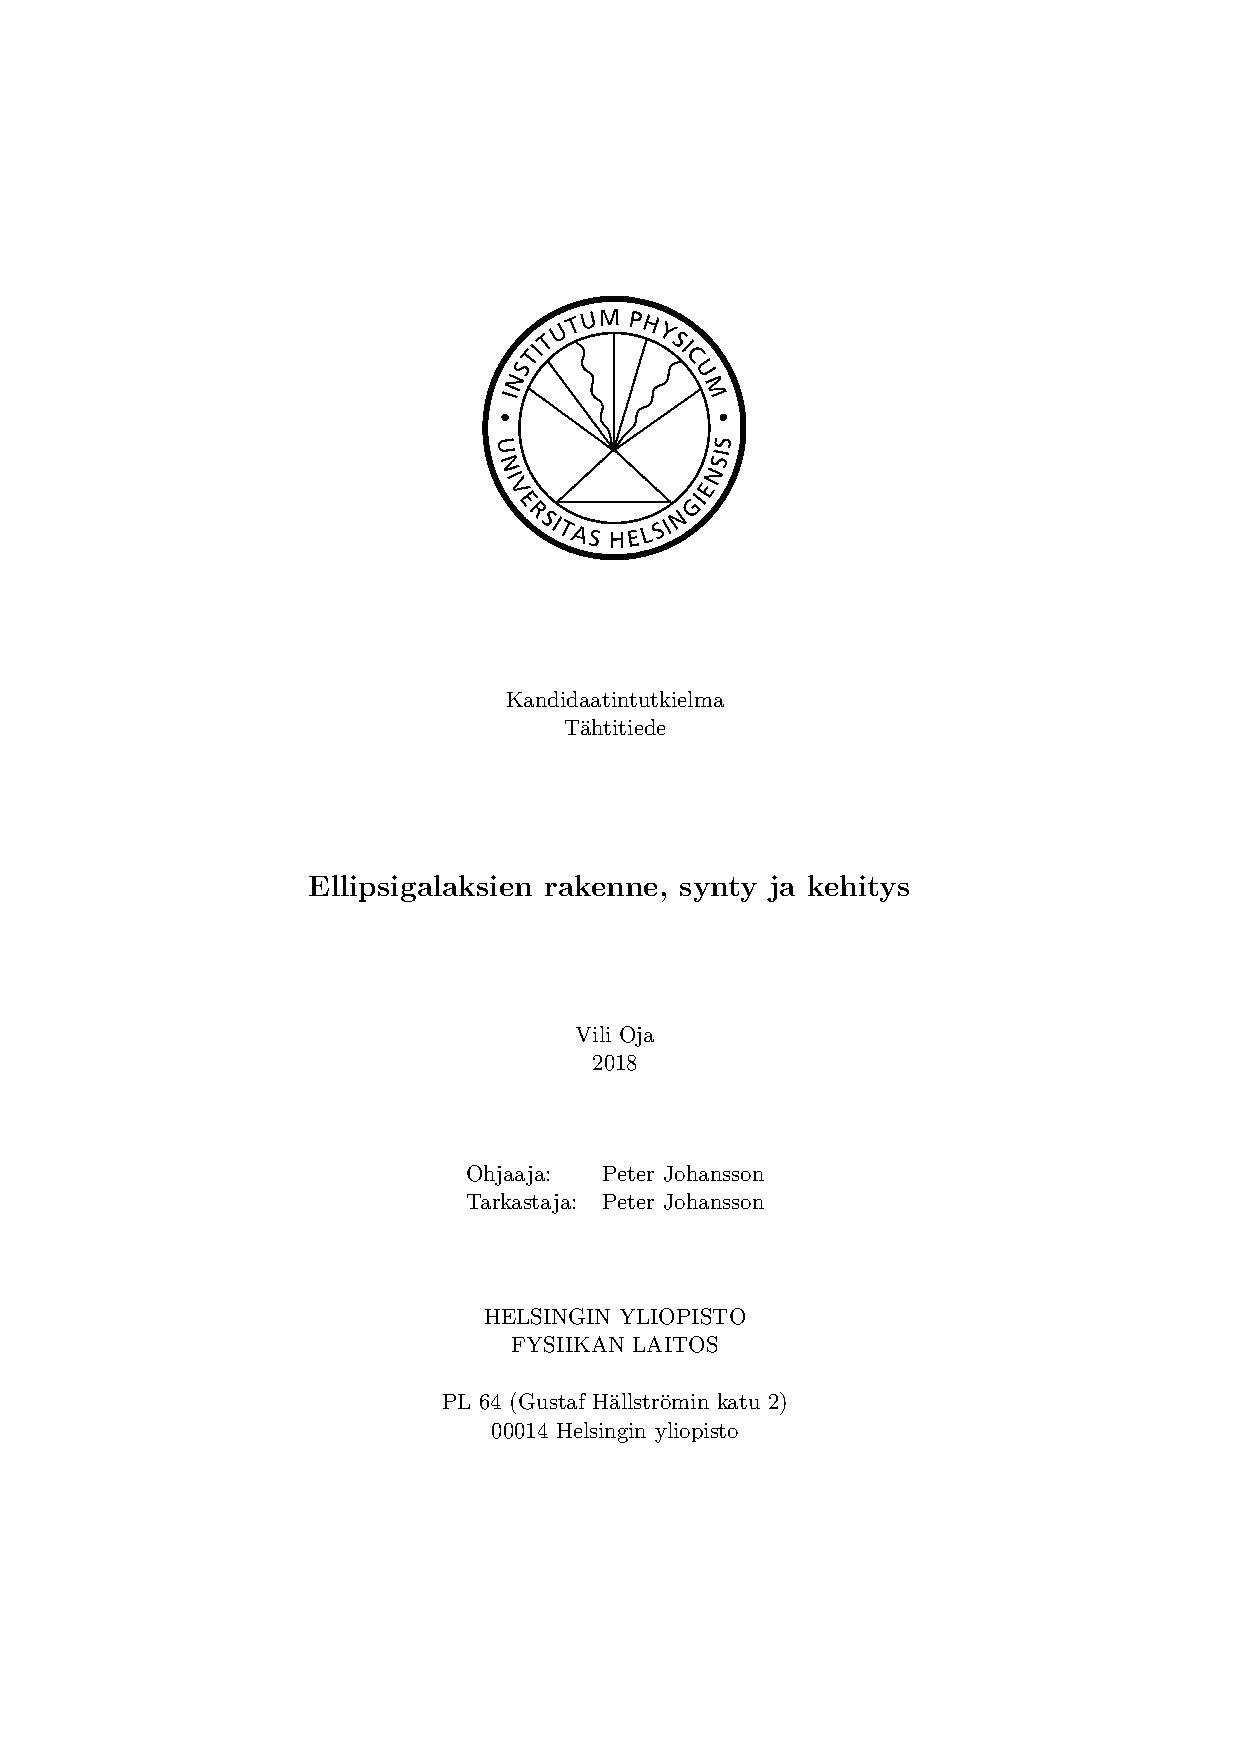
\includepdf[fitpaper]{../kansilehti/kansi.pdf}

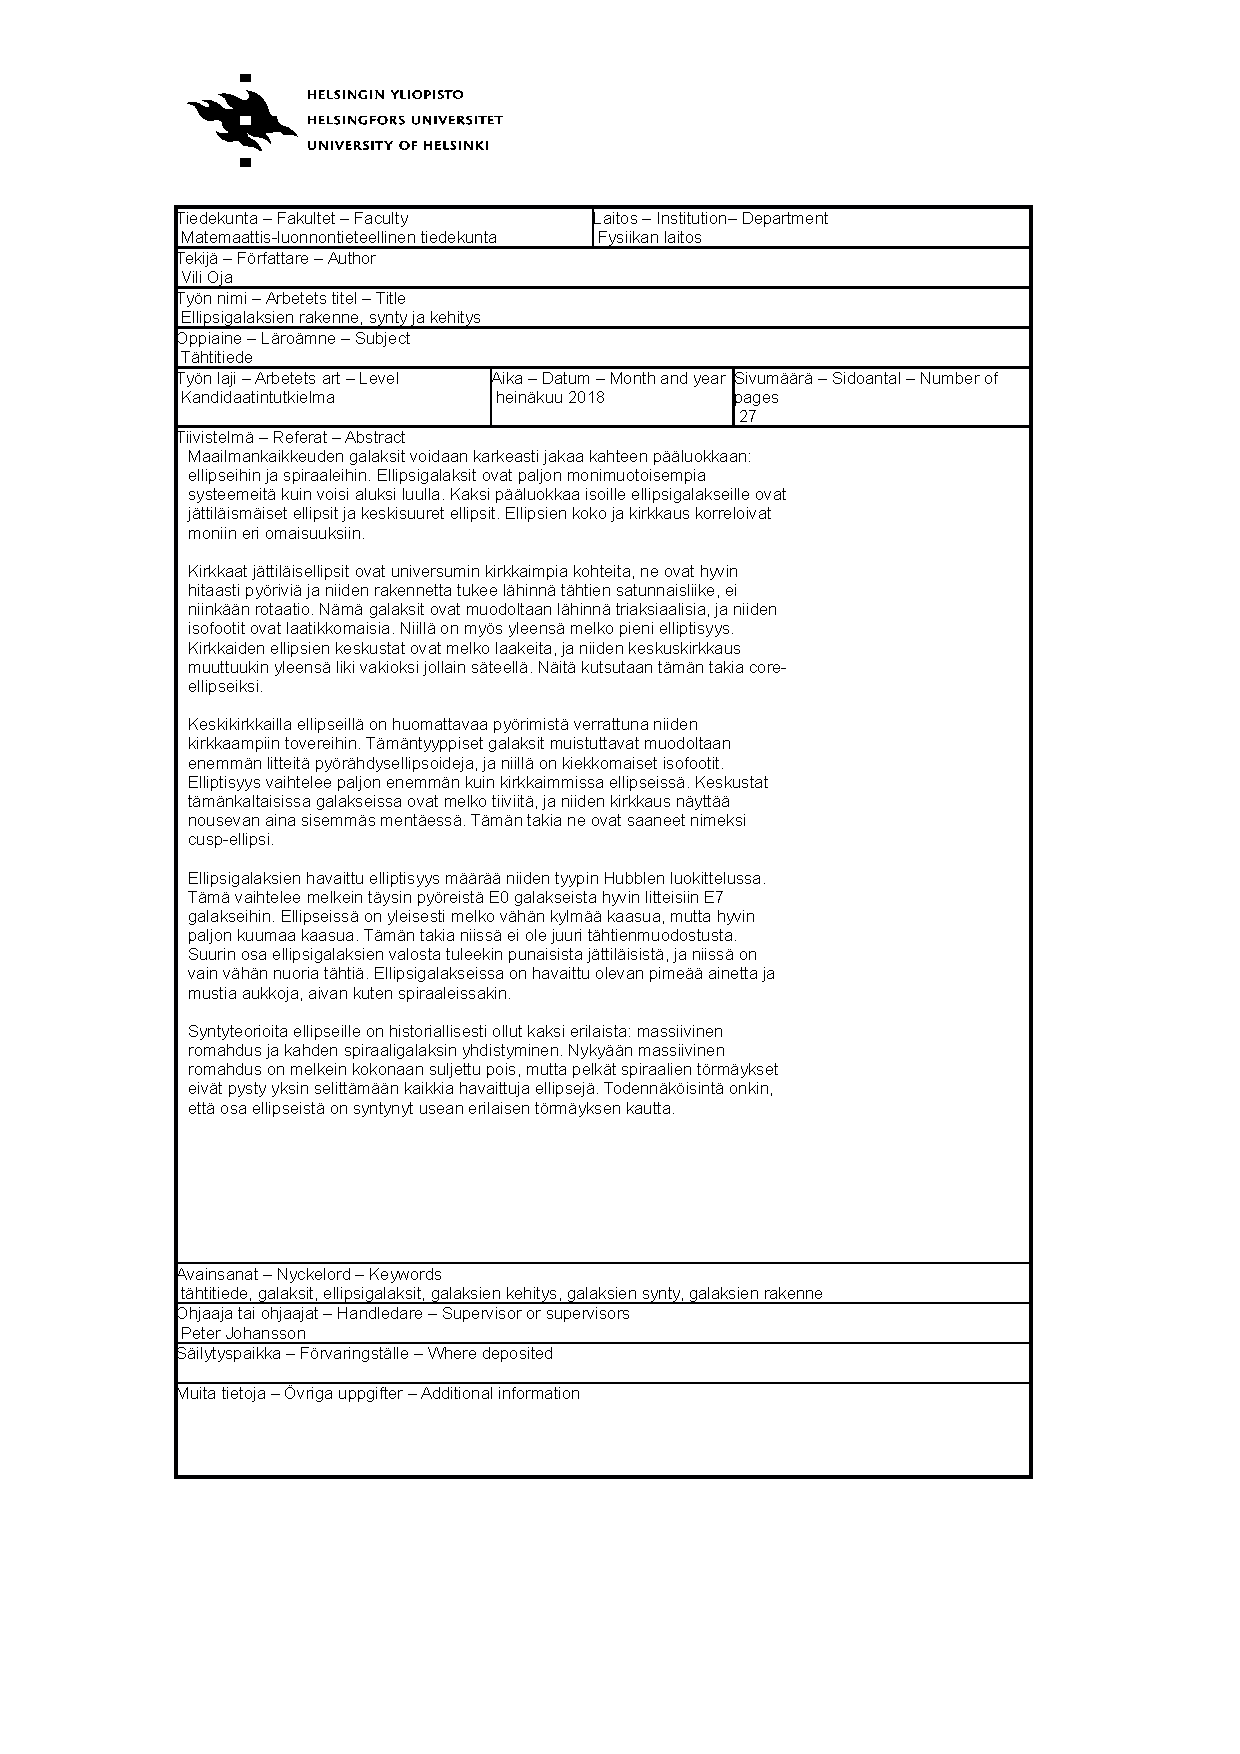
\includepdf[fitpaper]{../kansilehti/abstract.pdf}

% Sisällysluettelo
\newpage
\tableofcontents
\thispagestyle{empty}
\newpage
\setcounter{page}{1}
\parskip=1em \advance\parskip by 0pt plus 2pt
\pagestyle{fancy}
\cfoot{\thepage}

%%%%%%%%%%%%%%% Oleellinen sisältö alkaa%%%%%%%%%%%%%%%
\section{Johdanto}

Galaksit ovat dynaamisesti sidottuja järjestelmiä, jotka koostuvat tähdistä, tähtien jään\-teistä, kaasusta ja pölystä, ja jotka sijaitsevat pimeän aineen halojen keskellä. Ne ovat maailmankaikkeuden peruspalikoita, muodostaen galaksiryhmiä ja -joukkoja, universumin suurimpia näkyvän aineen rakenteita. Myös iso osa universumin tähtien muodostus tapahtuu niissä. Vallitseva tapa galaksien luokitteluun perustuu vanhaan Edwin Hubblen esittämään ``äänirautamalliin'', jossa galaksit jaoteltiin varhaisen (ellipsit) ja myöhäisen (spiraalit) tyypin galakseihin puhtaasti niiden optisen morfologian perusteella. Nimitykset ovat hieman harhaanjohtavia, sillä niillä ei ole mitään tekemistä galaksien todellisten muodostumisaikojen kanssa. Galaksit jaetaan siis elliptisiin, linssimäisiin, spiraaleihin sekä epäsäännöllisiin galakseihin. 

Iso osa galaksitutkimuksesta on keskittynyt spiraaligalakseihin, kuten oma Linnunratamme, mutta myös ellipsigalaksit ovat hyvin kiehtovia kohteita. Vaikka ne saattavat näyttää yksinkertaisilta, sitä ne eivät todellisuudessa ole. Ne ovat hyvin monipuolisia: nämä galaksit voivat olla litteitä pyörähdysellipsoideja tai sitten triaksiaalisia kappaleita. Triaksiaalisissa galakseissa on nimensä mukaisesti kolme riippumatonta akselia joiden ympäri tähdet voiva pyöriä. Osa ellipseistä pyörii jonkin verran kun osa ei taas pyöri juuri yhtään. Täytyy kuitenkin huomioida, että kaikki ellipsigalaksit pyörivät paljon hitaammin kuin spiraalit. Spiraaligalakseissa pyörimisnopeuden ja nopeusdispersion suhde on tyypillisesti kokoluokkaa $v_\mathrm{rot} / \sigma \sim 10-20$, kun taas suhteellisen nopeasti pyörivissä ellipseissä se on suuruusluokkaa  $v_\mathrm{rot} / \sigma \sim 1$, ja erittäin hitaasti pyörivissä ellipseissä vain $v_\mathrm{rot} / \sigma \lesssim 0.1$. Nopeusdispersiolla tarkoitetaan jonkin joukon kappaleiden (kuten galaksin tähtien) nopeuksien tilastollista hajontaa niiden nopeuksien keskiarvon ympärillä.

Ellipsigalaksit ovat myös kirkkaudessaan universumin ääripäitä: kirkkaat jättiläisellipsit ovat maailmankaikkeuden valovoimaisimpia galakseja, kun taas kääpiöellipsoidit ovat erittäin himmeitä. Yhteistä näille on vain suurpiirteinen muoto ja se, että niissä ei ole juuri lainkaan viileää kaasua ja vain vähän nuoria tähtiä. Ellipsigalakseissa on suhteellisesti erittäin vähän kylmää kaasua, minkä takia uusien tähtien muodostusta ei juuri ole. Kuumaa ionisoitunutta kaasua on puolestaan suhteessa paljon enemmän.

Yleisesti voidaan sanoa, että ellipsigalaksit ovat lievästi litteitä, soikeita systeemejä joita tukee tähtien satunnaisliike. Kaikissa galakseissa tähdet liikkuvat omilla radoillaan, mikä tukee järjestelmää, estäen sitä romahtamasta kasaan. Spiraaligalakseissa tähdet liikuvat pääosin samaan suuntaan toistensa kanssa kiekon tasossa, joten voidaan sanoa, että tähtien rotaatio tukee niitä. Ellipsigalakseissa puolestaan tähdet eivät liiku mihinkään yhteen tiettyyn suuntaan, vaan ne voivat olla hyvinkin erisuuntaisilla radoilla matkalla ympäri galaksia. Täten sanotaan, että tähtien satunnaisliike tukee ellipsigalakseja.

Voimme määrittää galaksin elliptisyyden pintakirkkauden tasokäyrän eli isofootin isoakselin puolikkaan $a$ ja pikkuakselin puolikkaan $b$ suhteesta, kaavalla $\varepsilon = 1 - b/a$. Elliptisyys pysyy keskimäärin vakiona galaksin halki, joten galakseja voi luokitella Hubblen tyypeiksi E$n$, missä $n = 10\varepsilon$. Tämä Hubblen tyyppi riippuu kuitenkin katselukulmasta, sillä osa ellipseistä on meitä kohti reuna edellä, kun taas osa näyttää litteän puolensa.

Kinematiikan ja fotometrian perusteella ellipsigalaksit voidaan jakaa karkeasti kolmeen luokkaan: kirkkaat jättiläismäiset ellipsit, keskikokoiset ellipsit, ja kääpiöellipsit. Kun ellipsistä tiedetään sen kirkkaus, muut ominaisuudet voidaan saada selville melko helposti, sillä nämä ominaisuudet riippuvat kirkkaudesta.

Kirkkaille ellipseille ($M_B \lesssim -20.5$) tyypillistä ovat vähäinen pyöriminen, laatikkomaiset isofootit, pieni elliptisyys ($\varepsilon \lesssim 0.3$) ja suhteellisen loivat keskustan kirkkausprofiilit. Keskikirkkailla ellipseillä ($-20.5 \lesssim M_B \lesssim -18$) puolestaan pyöriminen tukee niiden rakennetta merkittävästi, niillä on kiekkomaisia isofootteja, elliptisyys vaihtelee enemmän ($\varepsilon \lesssim 0.7$) ja keskustan kirkkausprofiileissa on jyrkkiä keskuspiikkejä. Himmeämmässä päässä ($M_B \gtrsim -18$) on kääpiöellipsejä ja kääpiösferoidaaleja. Niillä ei näytä olevan juurikaan pyörimistä ja niiden kirkkauskäyrät ovat kutakuinkin eksponentiaalisia. Massojen selville saamiseksi voimme hyödyntää viriaaliteoreemaa. Se kertoo miten keskimäärin kineettinen ja potentiaali-energia ovat tasapainossa. Mikäli galaksi on tasapainossa, voimme laskea tämän teoreeman avulla arvion massalle, kun tiedämme tähtien nopeudet.

Kun tutkailemme lähemmin galaksien keskusalueita, voimme huomata, että ellipsigalakseissa nopeusdispersio nousee keskelle mentäessä, ja tämän on yleisesti käsitetty johtuvan siitä, että keskustassa on supermassiivinen musta aukko, joka vaikuttaa voimakkaasti keskusalueen havaittaviin tähtiin. Ja kuten spiraaligalakseissa, myös ellipseissä on havaittu merkkejä pimeän aineen haloista. Epäsymmetriat ellipsigalaksien pinkakirkkauksissa antavat vihiä siitä, että ne ovat olleet osallisia galaksien törmäyksissä. Tämä kertoo mahdollisesta syntymekanismista.

Seuraavissa kappaleissa käsitellään ensin yleisesti ellipsigalaksien rakennetta; ja ominaisuuksia, ja sitten syvemmin erinäisiä teorioita ellipsien synnylle.

\section{Ellipsigalaksien rakenne}

\subsection{Yleisrakenne}
Yksi erittäin keskeinen käsite ellipsigalakseista puhuttaessa on efektiivinen säde $R_e$, joka määritellään säteenä jonka sisällä on puolet galaksin kirkkaudesta. Tämä on hyödyllinen, sillä ellipsien valo jakautuu hyvin laajalle alueelle, joten niille on vaikea määrittää mitään selvää ulkoreunaa. Toinen tähän liittyvä käsite on eksponentiaalinen skaalasäde $R_s$, jolla intensiteetti putoaa $e^{-1}$-kertaiseksi. Toisin kuin spiraaleissa, ellipseissä keskustan kirkkaus on tiiviisti linkittynyt kokonaiskirkkauteen. Kirkkaissa ellipseissa pätee, että mitä kirkkaampi galaksi on, sitä matalampi sen keskustan kirkkaus on ja sitä leveämpi sen ydin on.

Voimme käyttää Sérsicin empiiristä kaavaa kuvaamaan galaksin valon jakautumista.
\begin{equation}
I(R) = I(R_e) \ \mathrm{exp}\{-b[(R/R_e)^{1/n}]\} \ ,
\end{equation}
missä n on niin sanottu Sérsic indeksi. Muuttuja b valitaan siten että $R_e$ on tosiaankin efektiivinen säde. Jos $n>1$, $b \approx 1.999n - 0.327$. Jos n = 1 on kyseessä yksinkertainen eksponentiaalinen muoto. Jos n = 4 on kyseessä niinsanottu de Vaucouleursin laki, joka kehitettiin vartavasten kuvaamaan ellipsigalaksien valokäyriä. Sérsicin yleinen muoto kehitettiinkin tämän pohjalta. Keskustan ulkopuolella n = 4 kuvaa pintakirkkautta melko hyvin kirkkailla, keskisuurilla ellipseillä, kun vertaamme teoriaa havaintoihin. Mikäli havainnointi tapahtuu maapallon pinnalata, ilmakehän epätasaisuuksien aiheuttamat häiriöt eli seeing kuitenkin vaikuttaa voimakkaasti siihen kuinka laadukkaita kuvia voimme saada keskustasta. Avaruudesta havainnoitaessa tätä ongelmaa ei tietenkään ole. Kirkkaimmilla galakseilla keskustojen kirkkaus muuttuu melkolailla vakioksi jollain etäisyydellä. Himmeämmissä galakseissa keskustan kirkkaus näyttää nousevan niin pitkälle kuin instrumentit pystyvät sitä seuraamaan. Isoimmille ja kirkkaimmille galakseille sopii paremmin muodot joissa n on isompi. Pienimmille n $\approx$ 1 sopii melko hyvin \citep{galaxies}.

Himmeimmät ellipsit jakaantuvat kahteen ryhmään: kompakteihin ellipseihin sekä kääpiö\-ellipseihin ja -sferoidaaleihin. Kompakteilla on jonkin verran pyörimistä, kun taas kääpiö\-ellipsit eivät pyöri merkittävästi. Kaikkein himmeimmissä kohteissa aiemmin mainittu sääntö kirkkauden ja keskustan yhteydestä kääntyy päälaelleen: niissä keskustankin kirkkaus on suhteessa erittäin alhainen.

Ellipseissä on paljon tähtienvälistä ainetta, mutta sillä on hyvin erilaiset ominaisuudet kuin spiraaligalakseissa. Kuuma ($\sim 10^7$ K), röntgensäteitä emittoiva kaasu muodostaa suurimman osan tähtienvälistä ainetta. Tämän lisäksi useimmissa ellipsigalakseissa on lämmintä ($10^4$ K) ionisoitunutta kaasua ja kylmää ($<100$ K) kaasua ja pölyä. Kuumaa kaasua on tyypillisesti noin sata kertaa enemmän kuin kylmää kaasua, ja kylmää kaasua on noin sata kertaa enemmän kuin lämmintä kaasua \citep{schweizer:1987}. Toisin kuin spiraaleissa, pölyn ja kaasun määrät eivät korreloi kirkkauteen.

Litteälle pyörähdysellipsoidille kinemaattinen akseli, eli akseli jonka suuntaisesti havaittu pyörimisnopeus on nolla, osuu yhteen fotometrian pikkuaskelin kanssa. Osalla ellipseistä on kuitenkin havaittu olevan rotaatiota sekä iso- että pikkuakselin suhteen. Niiden kinemaattiset ja fotometriset akselit eivät siis täsmää. Tälläinen kinemaattinen epäkohdistus on yleisempää kirkkaammissa ellipseissä joita tukee nopeusdispersio. Tämä johtuu siitä, että triaksiaaliset potentiaalit tukevat tähtien ratoja, joilla on pyörimistä sekä ison että pienen akselin suhteen. Nopeasti pyörivissä ellipseissä sitä ei juuri havaita, mikä sopii yhteen sen käsityksen kanssa, että ne ovat aksisymmetrisiä \citep{levison:1987, statler:1987}.
 
Noin neljänneksellä ellipseistä on kinemaattisesti irtikytkeytynyt ydin (kinematically decoupled core (KDC)), jonka kulmaliikemäärävektori ei osu yksiin koko galaksin kanssa. Äärimmäisissä tapauksissa keskusta voi jopa pyöriä eri suuntaan kuin muu galaksi. Tällaiset ytimet on yleensä selitetty dynaamisesti erillisinä alijärjestelminä, jotka ovat jäämiä yhdistyneistä kumppaneista. Tälläinen kinemaattinen vääntyminen voi johtua myös ratojen projisoitumisesta, eikä välttämättä vaadi ydintä, joka on oma erillinen dynaaminen alijärjestelmänsä. Tämäntyyppisten ellipsien fotometria tai nopeusdispersioprofiilit eivät eroa merkittävästi tavallisesta, joten ei ole täysin selvää mikä on oikea syy tähän ilmiöön \citep{statler:1991, forbes:1995, carollo:1997}.

\subsection{Relaatiot}

Ellipsigalakseilla on tiukka empiirisesti havaittu yhteys keskustan nopeusdispersion, efektiivisen säteen ja efektiivisen säteen sisäisen pintakirkkauden välillä. Tämä on niin sanottu fundamentaalitaso (fundamental plane) \citep{djorgovski:1987, dressler:1987}. Se on yleisesti määritelty kaavalla
\begin{equation} \label{fundamentaalitaso}
 \mathrm{log} \, R_e = a \, \mathrm{log} \, \sigma_0 + b \, \mathrm{log} \, \langle I \rangle_e + \mathrm{vakio} \ .
\end{equation}
Muuttujat riippuvat hieman valitusta kaistasta. Tyypillisesti parhaan sovituksen parametrit ovat välillä $a \sim 1.2$ (sinisessä kaistassa) ja $a \sim 1.5$ (lähi-infrapuna kaistassa), ja $b \simeq -0.8$ (ei juuri riippuvuutta fotometrisestä kaistasta). Todellisen galaksin erovaisuutta näistä parhaan sovituksen arvoista sanotaan fundamentaalitason kallistumaksi. Tämä kallistuma kuvastaa todennäköisesti variaatioita galaksin massa-luminositeetti-suhteessa, mikä voi puolestaan johtua galaksin tähtipopulaation ominaisuuksista ja/tai pimeän aineen halon osuudesta \citep{capellari:2006}.

Ennen kuin fundamentaalirelaatio havaittiin, Faber \& Jackson huomasivat, että ellipsigalaksin luminositeetti korreloi sen keskustan nopeusdispersion kanssa kutakuinkin $L \propto \sigma^4_0$ \citep{faber-jackson:1976}. Tämä Faber-Jackson-relaatio on samanlainen kuin Tully-Fisher-relaatio spiraaligalakseille, joka siis on empiirisesti havaittu yhteys massan tai lumonositeetin ja kulmanopeuden välillä. Koska $L \propto \langle I \rangle_e R^2_e$, Faber-Jackson-relaatio implikoi fundamentaalitason relaatiota, jossa $a = 2$ ja $b = -1/2$. Nämä arvot ovat melko erilaisia havaitun fundamentaalitason relaation parhaista sovituksista, mikä osoittaa, että Faber-Jackson-relaatio ei aivan täysin vastaa fundamentaalitasoa.


\subsection{Isofoottien muotoja} \label{isofootit}
Ellipsigalaksien muoto riippuu katselukulmastamme. Koska näemme galakseja satunnaisista suunista, voimme muodostaa kuvan keskimääräisestä kolmiulotteisesta muodosta käyttämällä hyväksi näennäisten muotojen jakaumaa. Triaksiaalisissa ellipseissä isofoottien, eli pintakirkkauden tasokäyrien, litistyneisyys voi muuttua säteen funktiona, mitä sanotaan isofoottien vääntymiseksi. Ellipsigalaksien isofootit eivät myöskään yleensä ole täysin elliptisiä. Eroavaisuuksia täy\-del\-li\-ses\-tä ellipsistä voidaan kuvata seuraavan funktion Fourier'n kertoimilla
\begin{equation}
R_{iso}(\phi)-R_{ell}(\phi) = a_0 + \sum^\infty_{n=1}(a_n \mathrm{cos} (n \phi) + b_n \mathrm{sin} (n \phi)) \ ,
\end{equation}
missä $R_{iso}(\phi)$ on isofootin säde kulmalla $\phi$ ja $R_{ell}(\phi)$ on ellipsin säde samalla kulmalla. Yleensä tarkastellaan ellipsiä joka sopii isofoottiin niin hyvin, että kertoimet $a_0, a_1, a_2, b_1$ ja $b_2$ ovat kaikki nolla virherajojen sisällä. Erot tästä parhaan sovituksen isofootista ilmaistaan korkeamman asteen Fourier'n kertoimilla, joilla $n\geq 3$. Erityisen mielenkiintoisia ovat kertoimen $a_4$ arvot, sillä ne kertovat onko isofootti kiekkomainen (disky, $a_4 > 0$) vai laatikkomainen (boxy, $a_4 < 0$) \citep{bender:1988}. Kuvassa \ref{fig:isofootit} on hahmoteltu miltä erilaiset isofootit näyttävät. 

\begin{figure}[h!tb]
\centering
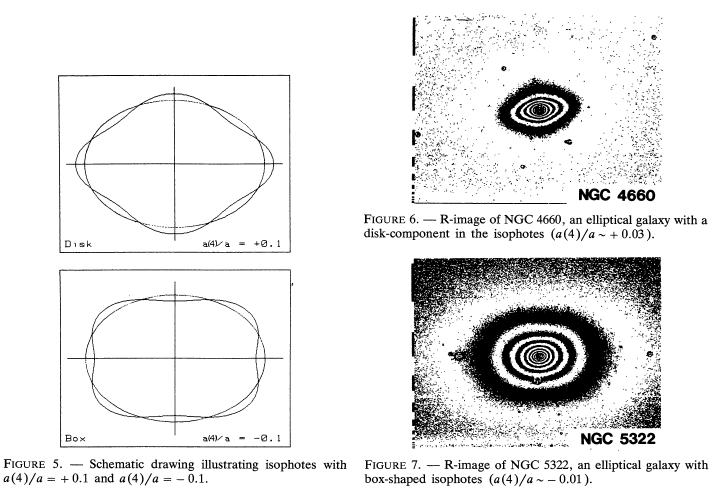
\includegraphics[width=\textwidth]{../kuvat/isofootit.png}
\caption{Kuvitus isofoottien eri muodoista, artikkelista \cite{bender:1988}. Vasemmalla ylhäällä on kiekkomainen isofootti ja sen alla laatikkomainen. Oikealla on kuvat oikeista galakseista joissa esiintyy näitä muotoja.}
\label{fig:isofootit}
\end{figure}
 
Toinen tapa kuvata isofootin eroja täydellisestä ellipsistä on määrittää kuinka paljon intensiteetti vaihtelee parhaan sovituksen ellipsillä
\begin{equation}
I(\phi) = I_0 + \sum^\infty_{n=1}(A_n \mathrm{cos} (n \phi) + B_n \mathrm{sin} (n \phi)) \ ,
\end{equation}
missä $I_0$ on parhaan sovituksen ellipsin intensiteetti. Kertoimet $A_n$ ja $B_n$ liittyvät kertoimiin $a_n$ ja $b_n$ seuraavasti:
\begin{equation}
A_n = a_n \left| \frac{\mathrm{d}I}{\mathrm{d}R} \right|, \ B_n = b_n \left| \frac{\mathrm{d}I}{\mathrm{d}R} \right| \ ,
\end{equation}
missä $R=a \sqrt{1-\varepsilon}$, jossa $\varepsilon$ on parhaan sovituksen ellipsin elliptisyys.

Erotus kiekkomaisten ja laatikkomaisten ellipsien välillä on tärkeä, sillä niissä löytyy systemaattisia eroja. Laatikkomaisissa on usein isofoottien vääntymistä. Tämä on mahdotonta aksisymmetrisille systeemeille, mutta tapahtuu luontaisesti jos galaksi on triaksiaalinen. Tämän takia kirkkaiden ellipsien usein ajatellaan olevan triaksiaalisia. Ne pyörivät hitaasti ja niissä on keskivertoa voimakkaampia radio- ja röntgenemissiotia.
 
Kiekkomaiset ovat himmeämpiä, niissä on suhteellisesti paljon pyörimistä ja vähän tai ei ollenkaan radio- tai röntgenemissioita. Nämä ovat yleensä keskikokoisia. Kiekkomaisilla ellipseillä taas ei puolestaan näy isofoottien vääntymistä juuri koskaan, mikä sopii yhteen käsityksen kanssa että ne ovat aksisymmetrisiä. 

Isofootin muoto myös korreloi ytimen ominaisuuksien kanssa, ja ellipsit voidaankin jakaa ytimen pintakirkkauden perusteella core-ellipseihin ja cusp-ellipseihin. Core-ellipseissä ytimen pintakirkkaus on melkein vakio, eli niiden keskustasta ``puuttuu valoa'' verrattuna tyypilliseen Sérsic profiiliin. Nämä galaksit ovat tyypillisesti isoja ja niiden keskustassa on massiivinen musta aukko. Nämä ovat laatikkomaisia. Cusp-ellipseissä puolestaan ytimen pintakirkkaus on hyvin suuri, eli niiden keskustassa on ``liikaa valoa'' verrattuna tyypilliseen Sérsic profiiliin. Nämä ovat yleensä pienimassaisempia ja pyörivät core-ellipsejä nopeammin. Nämä ovat tyypillisesti kiekkomaisia. Kuvassa \ref{fig:keskustat} näkyy kahden oikean galaksin keskusalueen pintakirkkauksia, joissa tämän kaksijakoisuuden voi nähdä. Todennäköisin syy tähän ilmiöön löytyy keskustojen supermassiivisista mustista aukoista. Kuten kappaleessa \ref{mergerit} tullaan tarkemmin toteamaan, massiiviset ellipsit syntyvät melko varmasti pienempien ellipsien yhteentörmäyksissä. Törmäyksissä mustat aukot uppoavat uuden galaksin keskellä, ja niiden dynaamiset vuorovaikutukset keskustan tähtien kanssa voivat levittää nämä tähdet laajalle alueelle, saaden aikaan odotetunlaisen core-ellipsin \citep{rantala:2018}.

\begin{figure}[h!tb]
\centering
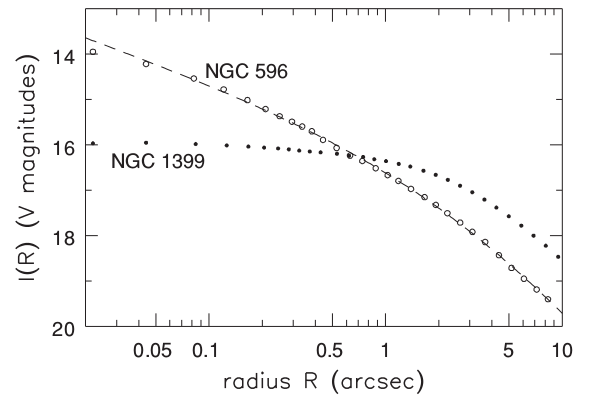
\includegraphics[width=\textwidth]{../kuvat/keskustat.png}
\caption{Kuvassa on kahden eri galaksin pintakirkkaudet V-kaistassa säteen funktiona. Jättiläismäisellä ellipsillä NGC 1399 ($M_V = -21.7$) näkyy selkeä keskusalue, jossa luminositeetti pysyy miltei vakiona (core-ellipsi). Puolet himmeämpi galaksi NGC 596 ($M_V = -20.9$) omaa puolestaan keskustaa kohti kasvavan pintakirkkauden (cusp-ellipsi). (Kuva 6.7. kirjasta \cite{galaxies}.)}
\label{fig:keskustat}
\end{figure}

%\subsection{Tähtien radat ja ominaisuudet}
%Toisin kuin spiraaligalakseissa, ellipsigalaksien tähtien rotaatio ei seuraa säännönmukaista kaavaa, vaan suurin osa niiden kineettisestä energiasta on satunnaisliikkeessä. Ja kuten spiraaligalaksien kirkkaus on yhteydessä niiden pyörimiseen, kirkkailla ellipsigalakseilla on suurempia nopeusdispersioita kuin himmeämmillä. Tämän yhteyden avulla voimme määrittää etäisyyksiä galakseihin. Tähtien radat voidaan jakaa pääsääntöisesti loop-ratoihin, joilla on jokin pyörimissuunta ja ne kiertävät galaksia, sekä box-ratoihin, jotka kulkevat galaksin keskustan läpi.
%
%Ellipsigalaksit pyörivät yllättävän hitaasti, mikä osoittaa, että tähdet eivät ole vielä relaksoituneet mihinkään lopulliseen tilaan, vaan niiden alkuperästä on vielä paljon pääteltävis\-sä. Galakseissa olevien tähtien ratanopeuksien määrittäminen on hankalaa, sillä toisin kuin kaasupilvissä, joissa voimme melko helposti katsoa emissioviivoja, tähdissä meidän täytyy katsoa absorptioviivoja. Nämä eivät yleensä ole siistejä ja kapeita atomiviivoja, vaan ne ovat itsessään leveitä. Viivan keskustan sijainnin lisäksi meidän täytyy huomioida myös viivan leveys ja muoto. Tämä vaatii korkeaa signaali-kohinasuhdetta ja pitkiä havaintoaikoja. Kaikkien galaksin tähtien valo on summa niiden yksittäisistä spektreistä. Jokainen spektri on Doppler-siirtynyt oman liikkensä mukaisesti, ja näiden rataliikkeiden takia tähtien yhteinen spektri on leveämpi ja matalampi kuin yksittäisten tähtien. Ellipsigalakseissa ei ole paljoa viileää kaasua, joten galaksin valo vastaa aika lailla tähtien emittoimaa valoa.
% 
%Kuten aiemmin mainittiin, ellipsigalakseilla on Faber-Jackson-relaatio, joka antaa karkean arvion kirkkauden ja nopeusdispersion yhteydelle. Voimme verrata tästä relaatiosta saatua todellisen kirkkauden arviota havaittuun kirkkauteen, ja saada siten arvion galaksin etäisyydelle. Galaksista tulleen valon kokonaismäärää on kuitenkin hankala määrittää, sillä iso osa siitä tulee galaksin himmeistä ulko-osista. Tämän takia Faber-Jackson-relaatiosta saadut arvot ovat vain melko suuntaa antavia. Tarkempi tapa on mitata halkaisija galaksin alueesta, jossa pintakirkkaus on keskiarvoltaan valitun suuruinen. Tiedämme, että keskuskirkkaus riippuu kokonaiskirkkaudesta, joten kun nyt tiedämme myös halkaisijan ja kirkkauden yhteyden, voimme muodostaa yhteyden nopeusdispersion ja halkaisijan välille. Tästä voimme saada etäisyysarvion kun tiedämme kuinka isolta galaksi näyttää Maasta katsottuna.
%
%Toisin kuin epäsäännöllisissä galakseissa ja spiraaligalakseissa, ellipseissä ei juuri näy kirkkaita sinisiä tähtiä. Kirkkaimpia tähtiä näissä galakseissa ovat sen sijaan HR-diagramman asymptoottihaaran jättiläiset. Vain vähän valosta on aallonpituudeltaan alle 3500 Ång\-strömiä, mikä osoittaa, että ellipsigalakseissa on syntynyt erittäin vähän tähtiä viimeisen parin miljardin vuoden aikana. Toisaalta vain tähdet joiden massa on alle 2 $M_\odot$ elävät yli miljardi vuotta, ja nämä tuottavat isoimman osan valostaan jättiläisvaiheessa. Joten ellipsigalaksien valo on pääosin peräisin punaisista jättiläisistä. Kuten aiemmin todettiin, ellipsigalaksien muut ominaisuudet ovat yhteydessä kirkkauteen. Samaten galaksin väri ja kirkkaus ovat linkittyneitä näkyvän valon alueella ja lähi-infrapunassa. Kirkkaammat galaksit ovat punaisempia ja himmeämmät sinisempiä. 
%
%Tähtipopulaatioita karakterisoi niiden tähtienmuodostushistoria (star-formation history, SFH), lähtömassafunktio (initial mass function, IMF) sekä kemiallisen rikastumisen historia. Varhaisen tyypin galakseille on havaittu väri-magnitudi-korrelaatio, eli niiden niiden väri korreloi vahvasti luminositeetin kanssa. Tämän perusteella ei voi kuitenkaan suoraan todeta mitään tähtipopulaation fysikaalisista ominaisuuksista, sillä ikä-metallisuus-degeneraatio haittaa tätä. Nuoret tähdet joilla on korkea metallisuus näyttävät samanlaisilta kuin vanhat tähdet joilla on vain vähän metalleja. Nykyään useat tutkimukset ovat samaa mieltä siitä, että relaatio värin ja magnitudin välillä johtuu pääosin metallisuudesta, ei iästä.
%
%Absorptioviivat antavat paremman kuvan tähtipopulaatioista, sillä niiden avulla päästään eroon edellä mainitusta degeneraatiosta. On havaittu, että osa viivoista ovat herkempiä iälle, kun taas osasta näkee paremmin populaation metallisuuden. Ellipsigalaksien tähtien iät näyttävät olevan laajalla välillä, noin kahdesta gigavuodesta aina universumin alkuajoille asti. Metallisuudet puolestaan näyttävät olevan aika pienellä välillä.

\subsection{Pimeä aine}
Spiraaligalakseissa neutraalin vedyn rotaatiokäyrät ovat vahva todiste pimeän aineen olemassaololle. Ellipsigalakseissa pimeän aineen tutkiminen on kuitenkin haastavampaa, sillä niissä ei ole yhtä hyviä ja helposti tulkittavia indikaattoreita isoilla säteillä. Yksi keino on käyttää hyväksi tähtien kinematiikkaa, jota saadaan integroidun valon absorptiospektroskopiasta. Ellipsien pintakirkkaus tippuu nopeasti säteen kasvaessa, joten tämä keino ei toimi kovin hyvin pitkillä etäisyyksillä. Mittauksia onkin pystytty tekemään enintään $\sim$2 efektiivisen säteen päähän. Tällä tavalla mitatut kinematiikat ovat näyttäneet, että tyypillisesti näkösäteen suuntainen nopeusdispersioprofiili on kutakuinkin vakio yhdestä efektiivisestä säteestä ulospäin. Tämä vastaa massa-valo-suhdeprofiilia joka kasvaa ulospäin, jollainen on odotettavissa mikäli systeemin ympärillä on pimeän aineen halo. Säteen suhteen vakiona pysyvä nopeusdispersio voi toisaalta olla myös merkki siitä, että nopeusdispersioanisotropia muuttuu enemmän tangentiaaliseksi säteen kasvaessa \citep{marel:1993}. Ellipsigalaksien keskusalueiden massa-valo-suhteiden perusteella voidaan sanoa, että yhden efektiivisen säteen sisällä keskimäärin  30\% massasta on pimeää ainetta \citep{gerhard:2001, capellari:2006}.

Yksi keino rajata massajakauma kinemaattisista havainnoista on ratkaista Jeansin yhtälöi\-tä. Nämä ovat yhtälöitä, jotka kuvaavat tähtien liikettä gravitaatiokentässä. Näille ei kuitenkaan yleisesti löydy yksiselitteisiä ratkaisuja, ja täytyykin tehdä joitain oletuksia ratkaisujen saamiseksi. Esimerkkinä voidaan tarkastella pallosymmetristä tilannetta, jossa olemme havainneet pintakirkkausprofiilin $I(R)$ ja projisoituneen nopeusdispersioprofiilin $\sigma_\mathrm{p}(R)$, missä $R$ on projisoitunut säde. Tässä pallosymmetrisessä tilanteessa ainoa epätriviaali Jeansin yhtälö on
\begin{equation}
\frac{1}{\rho} \frac{\mathrm{d}(\rho \langle v_r^2 \rangle)}{\mathrm{d}r} + 2 \beta \frac{\langle v_r^2 \rangle}{\mathrm{d}r} = -\frac{\mathrm{d} \Phi}{\mathrm{d}r} \ ,
\end{equation}
missä $\rho$ on massatiheys, $\Phi$ on potentiaali ja $\beta$ on anisotropiaparametri, joka määritellään kaavalla
\begin{equation}
\beta(r) \equiv 1 - \langle v_\theta^2 \rangle / \langle v_r^2 \rangle \ .
\end{equation}
Tämä siis kuvaa tangentiaalisten nopeuksien suhdetta radiaalisiin nopeuksiin, eli kuinka anisotrooppista tähtien liike on.

Koska $\mathrm{d}\Phi / \mathrm{d}r = GM_\mathrm{tot}(r)/r^2$, missä $M_\mathrm{tot}$ on säteen $r$ sisään jäävä kokonaismassa, voimme kirjoittaa Jeansin yhtälön muodossa
\begin{equation} \label{jeansmassa}
M_\mathrm{tot}(r) = - \frac{\langle v_r^2 \rangle r}{G} \left[ \frac{\mathrm{d \, ln} \, \rho}{\mathrm{d \, ln} \, r} + \frac{\mathrm{d \, ln} \, \langle v_r^2 \rangle}{\mathrm{d \, ln} \, r} + 2 \beta \right] \ .
\end{equation}

Massaprofiili riippuu siis sekä nopeuden keskiarvosta $\langle v_r^2 \rangle (r)$ ja anisotropiaprofiilista $\beta(r)$. Koska näkösäteen suuntainen nopeus saadaan kaavalla $v_\mathrm{los} = v_r \mathrm{cos} \, \alpha - v_\theta \mathrm{sin} \, \alpha$, missä $\mathrm{cos} \, \alpha = R/r$, voimme kirjoittaa 
\begin{equation}
\sigma^2_\mathrm{p}(R) = \frac{2}{I(R)} \int_R^\infty \left( 1 - \beta \frac{R^2}{r^2} \right) \frac{\rho \, r \, \langle v_r^2 \rangle}{\sqrt{r^2 - R^2}} \mathrm{d} r \ .
\end{equation}

Havaittava näkösäteen suuntainen nopeusdispersio $\sigma^2_\mathrm{p}(R)$ täten riippuu molemmista muuttujista $\langle v_r^2 \rangle (r)$ ja $\beta(r)$, eikä konaismassalle $M_\mathrm{tot}(r)$ ole uniikkia ratkaisua. Tämä ratkaisujen puuttuminen, jota kutsutaan usein massa-anisotropia degeneraatioksi, haittaa massa-valo-suhdeprofiilien määrittämistä \citep{galform}. Tätä degeneraatiota voi kuitenkin ainakin osittain rikkoa ottamalla huomioon systeemistä havainnoituja korkeamman asteen nopeusmomentteja \citep{marel:1993}.

Toinen tapa massajakumien tutkimiseen suurilla säteillä on käyttää hyväksi diskreettejä dynaamisia tracereitä, kuten pallomaisia tähtijoukkoja, planetaarisia sumuja tai satelliittigalakseja. Tracereitä voi seurata suurillekin säteille, mutta niiden säteittäisnopeuksien dynaaminen mallintaminen on hankalaa, sillä säteittäisnopeuksien mallintaminen kärsii samasta massa-anisotropia degeneraatiosta kuin integroitujen valomittausten tulkitseminen. Lisäksi sopivia tracereitä on melko harvassa, joten tarkkojen tulosten saaminen on haastavaa. 

Kolmas tapa on röntgenkartoituksen avulla. Kirkkaita ellipsejä ympäröi usein leveä korona kuumaa röntgensäteitä emittoivaa kaasua. Kaasu on tähdistä irronnutta kaasua jota supernovat ovat kuumentaneet. Kaasu jäähtyy hiljalleen jarrutussäteily kautta, emittoiden röntgensäteitä \citep{galdyn}. Mikäli oletamme, että kaasu on hydrostaattisessa tasapainossa, säteen $r$ sisään jäävä kokonaismassa saadaan kaavasta 
\begin{equation}
M_\mathrm{tot}(r) = - \frac{k_\mathrm{B} T(r) r}{\mu m_\mathrm{p} G} \left[ \frac{\mathrm{d \, ln} \, \rho}{\mathrm{d \, ln} \, r} + \frac{\mathrm{d \, ln} \, T}{\mathrm{d \, ln} \, r} \right] \ ,
\end{equation}
missä $k_\mathrm{B}$ on Boltzmannin vakio, $\mu = \rho /(n m_\mathrm{p})$ on kaasun keskimääräinen molekyylimassa, $m_\mathrm{p}$ on protonin massa, $\rho$ on massatiheys ja $n$ on hiukkasten numerotiheys \citep{galform}. Oletus tasapainosta ei pidä täysin paikkaansa. röntgenhalon sisäosat jäähtyvät tehokkaammin kuin ulko-osat, sillä jäähtyminen riippuu elektronitiheydestä \citep{galdyn}. Tämän takia sisäosissa onkin odotettavissa virtauksia, ja niitä on havaittukin \citep{musho:1994}. Oletus tasapainosta pitää silti melko hyvin paikkansa, joten sitä silti käytetään.

Vertaamalla tätä kaavaan \ref{jeansmassa}, voimme nähdä, että tämä hydrostaattinen yhtälö on hyvin samanlainen dynaamiseen yhtälöön. Tässä on nopeuksien sijasta kaasun lämpötila, ja anisotropiakerroin on nolla. Joillekin ellipseille sekä lämpötila että kaasun tiheys voidaan ratkaista, joilloin voidaan saada tulos kokonaismassalle.  Tällä tavalla saadut massa-valo-suhteet ovat kokoluokkaa $\sim 100 \mathrm{M_\odot / L_\odot}$ satojen kiloparsekkien skaaloilla, mikä on vahvaa näyttöä pimeän aineen olemassaololle \citep{forman:1985, musho:1994}. Röntgenkartoitus ei myöskään kärsi samasta massa-anisotropia degeneraatiosta kuin kinemaattiset mallinnukset.


\subsection{Mustat aukot}

Nykyään on yleisesti hyväksytty, että lähes jokaisessa jättimäisessä ja keskikirkkaassa ellipsigalaksissa on supermassiivinen musta aukko sen keskellä \citep{kormendy:1995, ferrarese:2005}. Voimme havaita mustia aukkoja epäsuorasti katsomalla keskustassa olevien tähtien liikkeitä. Mikäli keskustan tähtien nopeusdispersiot ovat paljon suurempia kuin muualla niiden ympäristössä, voimme päätellä, että keskellä täytyy olla jokin hyvin massiivinen kohde. Tämä ilmiö on huomattu spiraaligalakseissa, ja havainnot näyttävät sen pätevän myös ellipsigalakseissa, mikä antaisi olettaa, että niissäkin on keskustassa massiivinen musta aukko. Isoimmat keskusmassat on löydetty galakseista joissa on isoimmat nopeusdispersiot. Musta aukko vuorovaikuttaa ympäröivän materian kanssa merkittävästi vain suhteellisen pienellä säteellä, joka voidaan määrittää kaavalla
\begin{equation}
r_{\mathrm{BH}} = \frac{G M_{\mathrm{BH}}}{\sigma^2} = 10.8 \mathrm{pc} \left( \frac{M_{\mathrm{BH}}}{10^8 \mathrm{M_\odot}} \right) \left( \frac{\sigma}{200 \mathrm{km/s}} \right)^{-2} \ ,
\end{equation}
missä $\sigma$ on galaksin keskustan tähtien karakteristinen nopeusdispersio. Tämän takia mustien aukkojen tutkiminen vaatiikiin erittäin tarkkoja havaintoja, jotta näin tarkka resoluutio voidaan saavuttaa \citep{galform}.

Mustia aukkoja on etsitty paljon läheisistä galakseista kinemaattisten tutkimusten avulla. Erityisesti yritetään löytää näyttöä massa-valo-suhteen kasvusta galaksien keskustassa mitä ei voida selittää tavallisilla tähtipopulaatioilla. Tämä voi osoittaa supermassiivisen mustan aukon olemassaolosta, mutta se voi johtua myös isosta määrästä himmeitä kohteita, kuten ruskeita kääpiöitä tai tähtien jäänteitä. Kuitenkin jos havaittu massa-valo-suhde on tarpeeksi iso ja rajoittuu tarpeeksi pienelle alueelle, voidaan nämä muut vaihtoehdot rajata pois sillä perusteella, että niillä olisi paljon galaksin ikää pienemmät eliniät \citep{maoz:1998}. Tämä johtuu siitä, että pienelle alueelle keskittynyt monen kappaleen järjestelmä lopulta hajoaa joko kappaleiden poistuessa järjestelmästä gravitaatiovuorovaikutusten takia, tai kappaleiden hajotessa fyysisten törmäysten seurauksena. Tähtien kinematiikan lisäksi mustia aukkoja voi joissain tapauksissa havaita myös aukkoja ympäröivän ionisoituneen kaasun kiekoista. Vaikka kaasun pyörimisnopeudesta voi saada periaatteessa hyvin tarkkoja rajoja sen sisällä olevalle massalle, kaasu on kuitenkin herkkää muillekin voimille kuin pelkälle gravitaatiolle, joten havaintojen tulkitseminen ei ole helppoa \citep{harms:1994, marel:1998}.
 
Kuten aiemmmin mainittiin, monilla ellipsigalakseilla on nopeusdispersioprofiilit, jotka nousevat jyrkästi keskustaa kohti. Yksinkertaisten isotrooppisten mallien sovittaminen osoittaa massa-valo-suhteen kasvua keskustassa, mikä sopii yhteen supermassiivisen mustan aukon olemassaolon kanssa. Tämä ei ole kuitenkaan yksiselitteistä, sillä sama massa-anisotropia joka on ongelmana halojen tutkimisessa haittaa myös tätä työtä. Keskustan nopeusdispersio voi olla suuri myös systeemissä, jossa ei ole suurta mustaa aukkoa jos keskusta on säteittäisesti anisotrooppinen. Tämä epäselvyys voidaan kuitenkin melko hyvin poistaa mittaamalla koko galaksin näkösäteen suuntainen nopeusjakauma (line-of-sight velocity distribution, LOSVD). Tämä tarkempi data yhdistettynä kehittyneisiin malleihin on antanut vahvaa näyttöä supermassiivisille mustille aukoille muutamassa tusinassa läheisessä ellipsigalaksissa. 

Kun havaintodatan määrä mustista aukoista on kasvanut, on voitu alkaa tehdä johtopäätöksiä korrelaatioista mustan aukon massan ja galaksin muiden ominaisuuksien välillä. Mustan aukon koko korreloi esimerkiksi sferoidin luminositeetin kanssa. Vielä tiukempi yhteys löytyy mustan aukon massan ja sferoidin nopeusdispersion välillä, joka määritellään kaavalla 
\begin{equation}
M_{\mathrm{BH}} = (1.3 \pm 0.2 ) \times 10^8 \mathrm{M_\odot} \left( \frac{\sigma_\mathrm{e}}{200 \mathrm{km/s}} \right)^\gamma \ ,
\end{equation}
missä tekijä $\gamma$ on välillä 3.75 ja 4.8, riippuen käytetystä datasta ja siitä, kuinka isolta alueelta nopeusdispersio on mitattu \citep{gebhardt:2000, ferrarese:2000}. Yhtä tiukkoja relaatioita on havaittu myös mustan aukon massan ja ellipsin kokonaismassan välillä, sekä mustan aukon massan \citep{haring:2004} ja galaksiin sopivan Sérsic indeksin välillä \citep{graham:2001}. Nämä korrelaatiot antavat viitteitä siitä, että mustan aukon muodostus on hyvin kytkeytynyt itse galaksin sferoidaaliosan muodostumiseen.

\section{Ellipsigalaksien syventävä teoria}

Tämä kappale keskittyy syvemmin ellipsigalaksien erilaisiin syntyteorioihin ja niihin vaikuttaviin havaintoihin. Vaikka teorioita galaksien muodostumiselle testataan simulaatioilla, on kaikki saamamme tieto kuitenkin pohjimmiltaan lähtöisin havainnoista. Katsomalla taivaalle voimme mitata sekä galaksien ominaisuuksia että nähdä menneisyyteen, miltä tilanne näytti kun maailmankaikkeus oli nuorempi. 

\subsection{Ehdotettuja syntyteorioita}

Ellipsigalaksien dynaaminen rakenne on paljon vähemmän järjestäytynyt kuin kiekkomaisten galaksien, mikä antaa viitteitä siitä, että niiden muodostuminen oli paljon rajumpaa. Kaikki ellipsigalaksien muodostumisteoriat olettavatkin, että rajulla relaksaatiolla (violent relaxation) oli tärkeä osa jossain vaiheessa muodostumisprosessia. Rajulla relaksaatiolla tarkoitetaan muutosta yksittäisten kappaleiden energioissa gravitaatiopotentiaalin vaihtelujen takia.

Kun tähti liikkuu vakioisessa potentiaalissa $\Phi$, sen energia $E = \frac{1}{2} v^2 + \Phi$ ei muutu. Mutta mikäli potentiaali $\Phi(\textbf{x}, t)$ muuttuu paikan ja ajan funktiona, energia ei ole vakio, vaan muuttuu kaavan \ref{violrelax} mukaisesti \citep{galdyn}.
\begin{equation} \label{violrelax}
\frac{\mathrm{d}E}{\mathrm{d}t} = \frac{\partial \Phi}{\partial t}
\end{equation}
Kuten kaavasta nähdään, tämä relaksaatio ei riipu kappaleen massasta, joten raju relaksaatio ei erottele kappaleita systeemissä niiden massan perusteella. Aikaskaala rajulle relaksaatiolle on samaa luokkaa vapaan pudotuksen aikasakaalan kanssa \citep{bell:1967}, joka on aika, joka systeemiltä kuluisi romahtaa jos siihen vaikuttaisi vain sen oma gravitaatio. Raju relaksaatio tapahtuu siis suhteellisen nopeasti, mistä sen nimikin on peräisin. Simulaatiot ovat kuitenkin osoittaneet, että raju relaksaatio ei yleisesti ottaen ole koskaan ``valmis'', vaan hiukkasten loppuenergiat korreloivat niiden alkuarvojen kanssa, ja systeemin lopullisen muodon perusteella voi tehdä päätelmiä sen alkutilasta \citep{aarseth:1978, white:1978, albada:1982, may:1984}.

Käytännössä tämä siis tarkoittaa, että galaksin eri osat sekoittuvat lähes kokonaan keskenään. On havaittu, että raju relaksaatio joko kylmän ja epäsymmetrisen alkutilan romahtamisen aikana tai kahden suunnilleen samanmassaisen kohteen yhdistymisen jälkeen tuottaa  ellipsoidimaisia systeemejä, joiden tiheysprofiilit täsmäävät ellipsigalakseja.

Ellipsigalaksien muodostumiselle onkin historiallisesti ollut kaksi kilpailevaa teoriaa: massiivinen romahdus ja kahden galaksin yhdistyminen \citep{galform}. Ensimmäisessä mallissa galaksi muodostuu lyhyehköllä aikaskaalalla kun sen tarkemmin määrittelemätön alkutilanne romahtaa ja virialisoituu. Tässä tähdet muodostuvat samaan aikaan kuin itse lopullinen galaksikin. Jälkimmäisessä mallissa ellipsigalaksi muodostuu kun kaksi kiekkomaista galaksia törmää ja yhdistyy. Tässä tapauksessa tähtien synty ei tapahdu samanaikaisesti itse ellipsin muodostumisen kanssa. Kuvassa \ref{fig:muodostus} on havainnollistettu eroja eri skenaarioiden aikaskaalojen välillä.

Kumpikaan näistä skenaarioista ei täysin yksin vastaa nykyistä käsitystä ellipsigalaksien muodostumiselle. On kuitenkin hyvä käydä läpi mikä niissä toimii ja mikä ei, millaisia lopputuloksia nämä kaksi eri tapaa antavat ja miten ne sopivat yhteen nykykäsityksen kanssa.

\begin{figure}[h!tb]
\centering
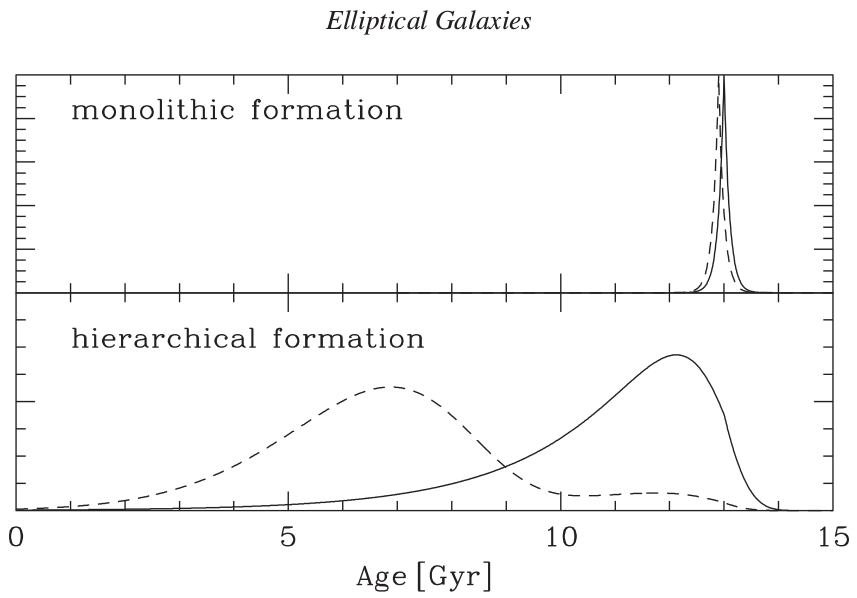
\includegraphics[width=\textwidth]{../kuvat/formation.png}
\caption{Kuvassa näkyy erot monoliittisen romahduksen (ylempi ruutu) ja mergerin (alempi ruutu) ellipsigalaksipopulaation muodostumisen välillä. Kiinteä viiva kuvaa keskimääräistä tähtienmuodostushistoriaa, kun taas katkoviiva näyttää baryonisen massan keskimääräisen kasvunopeuden suurimmassa galaksin edeltäjässä. Romahdusskenaariossa tähtien oletetaan muodostuvan lyhyessä kertarysäyksessä ja muodostovan galakseja samanaikaisesti tai piakkoin tämän jälkeen. Galaksien yhdistymisskenaariossa tähdet muodostuvat pidemmällä aikajaksolla useammassa jo olemassaolevassa galaksissa, ja ne yhdistyvät vasta paljon myöhemmin nykyään havaittaviksi ellipseiksi. (Kuva 13.4. kirjasta \cite{galform}.)}
\label{fig:muodostus}
\end{figure}

\subsubsection{Monoliittinen romahdus}

Massiivisessa tai `monoliittisessa' romahduksessa ellipsigalaksi syntyy korkealla punasiirtymällä yhdessä intensiivisessä purskauksessa tähtienmuodostusta. Tätä seuraa galaksin tähtipopulaation passiivinen kehitys nykypäivään saakka, eli galaksit eivät koe massiivisia törmäyksiä, ja niiden tähdet kehittyvät eteenpäin ilman sen erikoisempia tapahtumia \citep{partridge:1967, larson:1975}. Motiivina tälle selitykselle oli, että ellipsigalaksit näyttävät hyvin homogeenisiltä ja niillä on hyvin yhtenäiset tähtipopulaatiot. Tämänlaisen ellipsin lopullinen muoto riippuu siitä, miten paljon se säteilee energiaa pois romahduksessaan, eli kuinka dissipatiivinen romahdus on.

Mikäli systeemissä ei tapahdu juuri ollenkaan dissipaatiota, käytännössä kaikki kaasu voi muuttua tähdiksi romahduksen aikana tai hyvin pian sen jälkeen. Mallit pallomaiselle romahdukselle antavat tässä tapauksessa tulokseksi, että ellipsien olisi täytynyt muodostua yli punasiirtymillä z = 20, mikä sotii voimakkaasti nykykäsitystä vastaan, että vain pieni osa tähtiä syntyi ennen punasiirtymää z = 6. Eräs toinen seikka energiahäviöttömässä mallissa on se, että raju relaksaatio ei tee eroa pimeän aineen ja tähtien välillä, joten se ei voi erottaa niitä. Tämä ei sovi yhteen havaintojen kanssa, joiden mukaan pimeä aine on keskittynyt galaksien ulko-osiin, ja keskempänä on vain tähtiä \citep{galform}.

Koko tilanne on kuitenkin erilainen mikäli systeemi on dissipatiivinen romahtaessaan. Tällöin tähdet muodostuvat aikaskaalalla, joka on pidempi kuin romahtamisen aikaskaala. Kaasu ja pimeä aine voivat paremmin erottua, jolloin vältytään edellä mainitulta ongelmalta jossa olemme havainneet pimeää ainetta vain galaksien ulko-osissa. Koska tähtien muodostus on levinnyt paljon pidemmälle aikavälille, myöhemmin syntyvät tähdet ovat metallirikkaampia kuin ensimmäisinä syntyneet. Tästä voi seurata samanlaisia metallisuuden gradientteja kuin todellisissa ellipseissä on havaittu \citep{larson:1974}.

Vaikka tämä näyttää paremmalta kuin ensimmäinen malli, on siinäkin omat ongelmansa. Mikäli ellipsit olisivat syntyneet romahduksessa, mikä erottaa ne spiraaligalakseista? Miksi toisessa tapauksessa kaasun pyöriminen jää tukemaan galaksin rakennetta mutta toisessa ei? Tämä vaatisi joko että ellipsien protogalakseilla on palon pienemmät kulmaliikemäärät, tai sitten että ellipseissä baryonisen aineen kulmaliikemäärä siiryy paljon tehokkaammin pimeään aineeseen. Simulaatiot osoittavat, ettei ole kuitenkaan aivan mahdotonta, että ellipseillä liikemäärän siirtyminen olisi tehokkaampaa \citep{katz:1991, katz:1992}.

Isoin ongelma suoralle romahtamiselle on kuitenkin oletus siitä, että itse galaksin muodostus tapahtuisi samalla kun iso osa tähdistä syntyy melko lyhyessä ajassa. Suurimmalla osalla normaaleista ellipseistä näyttää olevan hyvin vanhat tähtipopulaatiot joiden keskimääräinen ikä on 10 miljardin vuoden paikkeilla. Tämä tarkoittaisi, että muodostumisen olisi täytynyt tapahtua kun z $\gtrsim$ 2 ja galaksit olisivat varttuneet passiivisesti sen jälkeen. On kuitenkin havaittu, että punasiirtymän z $\sim$ 1 kohdalla suhteellisen massiivisiset, passiivisesti kehittyvät galaksit olivat 3-4 kertaa tiheämpiä kuin nykypäivänä \citep{bell:2004, brown:2007, faber:2007, taylor:2009}. Eli isoin osa ellipsigalakseista muodosti tähtiä tai ei ollut vielä kasautunut lopulliseen muotoonsa punasiirtymän z = 1 kohdalla. Myös ellipsien koko oli noihin aikoihin paljon pienempi kuin samanmassaisilla galakseilla nykyään \citep{daddi:2005, trujillo:2006, dokkum:2008, wel:2008}. Tämä käytännössä sulkee monoliittisen romahtamisen kokonaan pois ainoana syntymekanismina. Tähän liittyy myös termi galaktinen supistuminen eli downsizing, joka viittaa antikorrelaatioon galaksin massan ja tähtien muodostumisiän välillä. Massiivisimmissa galakseissa on vanhempia tähtiä kuin pienemmissä galakseissa \citep{johansson:2012}.

\subsubsection{Mergerit} \label{mergerit}

Galaksien yhdistymiset eli mergerit ovat toinen ehdotus ellipsien synnylle. Äärimmäisessä tapauksessa tämä hypoteesi olettaa, että lähes kaikki tähtienmuodostus tapahtuu galaksien kiekoissa, ja että aivan kaikki ellipsit syntyvät kiekkogalaksien yhdistymisistä. Ensimmäinen väite on mahdollinen, sillä läheisen maailmankaikkeuden tähtienmuodostus on rajoittunut pääasiaalisesti galaksien kiekkoihin sekä tähtipurkausgalakseihin (starburst-galaxy). Tähtipurkausgalaksit ovat nimensä mukaisesti galakseja, joissa on merkittävää tähtienmuodostusta. Omassa Linnunradassamme syntyy tähtiä noin 3 $M_\odot$/yr, kun taas tähtipurkausgalakseissa tähtiä voi muodostua jopa 100 kertaa nopeammin \citep{extragal}. Esimerkiksi juuri galaksien törmäyksissä syntyy tähtipurkausgalakseja.

Jälkimmäinen pointti, että kaikki ellipsit muodostuisivat törmäyksissä, ei välttämättä kuitenkaan sovi yhteen havaintojen kanssa. Selvää kuitenkin on, että mergereitä tapahtuu. Ongelmana on, että voiko oikeiden havaittujen galaksien muodostumisesta syntyä galakseja jotka muistuttavat nykypäivän ellipsejä, ja voiko yhdistymisiä tapahtua tarpeeksi paljon ja oikeanlaisissa ympäristöissä, jotta saamme samanlaisen ellipsipopulaation kuin mitä nykyään havaitaan. Kuvassa \ref{fig:antenni} näkyy ehkä tunnetuin mergeri ja tähtipurkausgalaksi, Antennigalaksit.

\begin{figure}[h!tb]
\centering
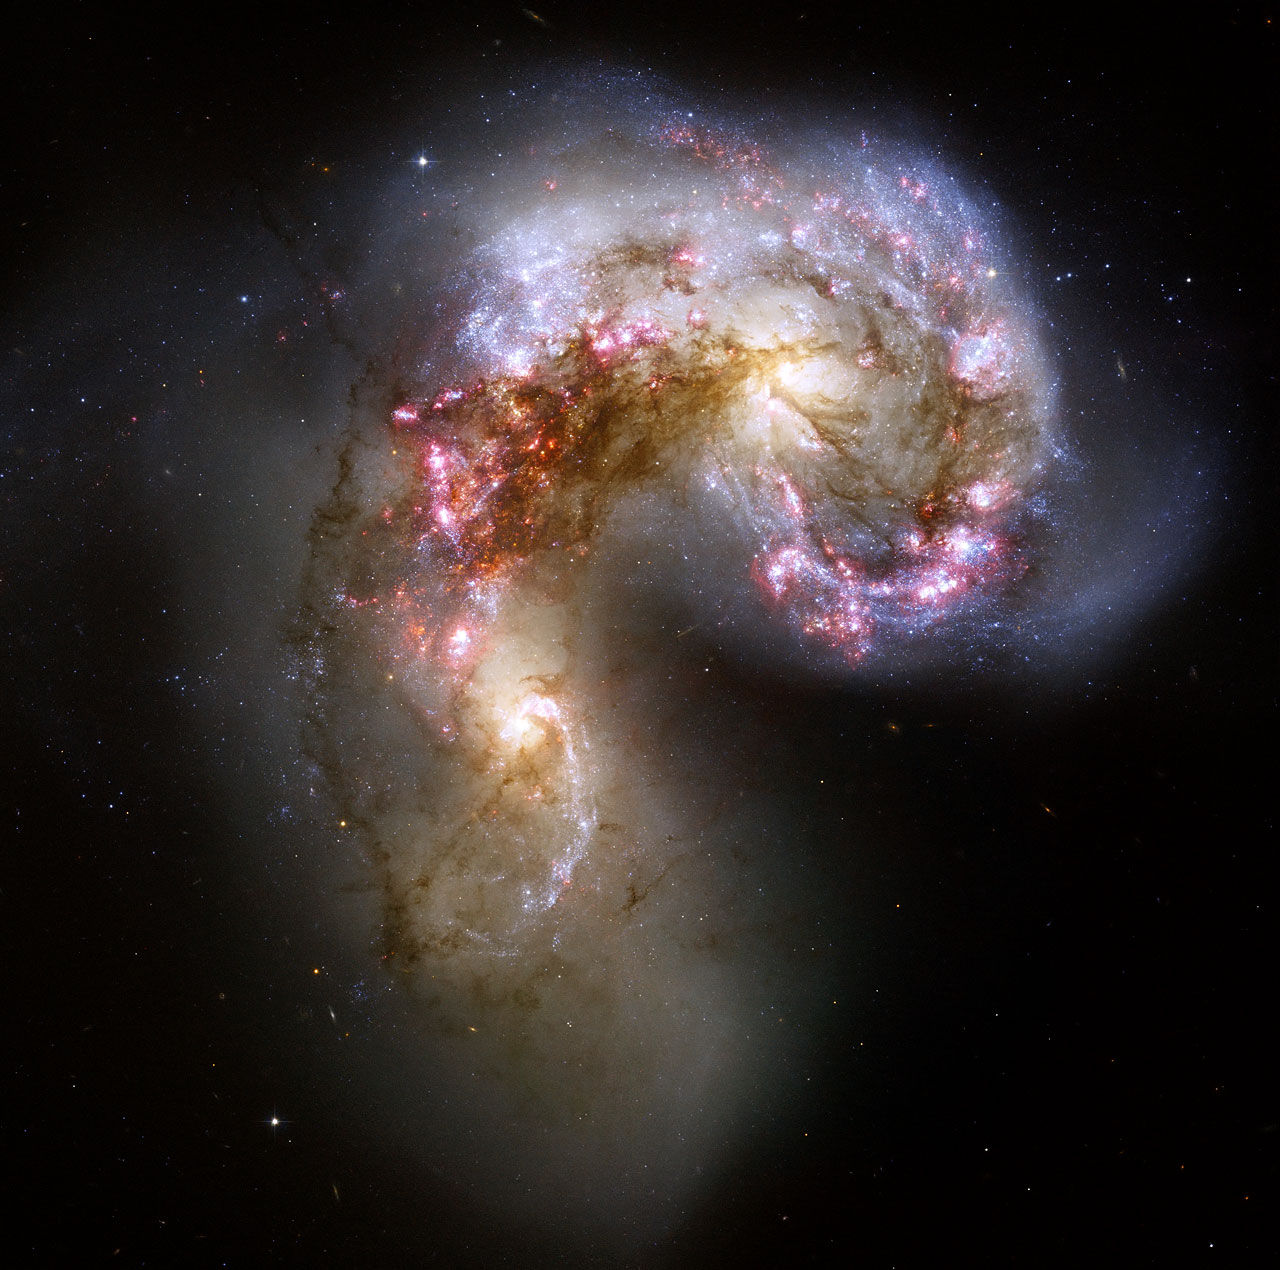
\includegraphics[width=\textwidth]{../kuvat/antenni.jpg}
\caption{Hubblen ottama kuva Antennigalakseista. Galaksit NGC 4038 (vasemmalla) ja NGC 4039 (oikealla) ovat noin 20 megaparsekin päässä meistä, ja ne törmäsivät toisiinsa ensimmäistä kertaa noin 500 miljoonaa vuotta sitten. Niiden ydinten on arvioitu yhdistyvän noin 80 miljoonan vuoden kuluttua \citep{lahen:2018}. Galaksissa on nähtävissä voimakasta tähtienmuodostusta, kuten on odotettavissa kun kaksi kaasurikasta kiekkogalaksia törmäävät toisiina. Myös galaksien morfologia on hyvin ainutlaatuinen törmäyksen seurauksena. (Kuva: NASA/ESA)}
\label{fig:antenni}
\end{figure}

Aikaisimmissa simulaatioissa tutkittiin tähtikiekkoja pienimassaisten pimeän aineen halojen sisällä, minkä seurauksena syntyneet galaksit pyörivät aivan liian nopeasti verrattuna havaintoihin \citep{gerhard:1981, farouki:1982, negroponte:1983}. Kun halojen kokoa ja massaa kasvatettiin, huomattiin, että lopulliset galaksit pyörivät hitaammin \citep{barnes:1988}. Syy tälle löytyy dynaamisesta kitkasta. 

Dynaamisella kitkalla tarkoitetaan ilmiötä, jossa jokin hiukkaskentässä liikkuva kappale vetää puoleensa ympäröiviä hiukkasia. Gravitaation takia nämä hiukkaset muodostavat massatihentymän liikkuvan kappaleen perään, vetäen sitä enemmän puoleensa ja siten hidastaen sen liikettä. Kuvassa \ref{fig:dynkitka} on havainnollistus ilmiöstä. Dynaamisen kitkan voimakkuus galaksien yhdistymisessä on verrannollinen galaksien massatiheyteen. Chandrasekharin kaava dynaamiselle kitkalle on
\begin{equation}
\mathrm{F_{df}} = - 4 \pi \left( \frac{G M_S}{v_S} \right)^2 \mathrm{ln} \Lambda \, \rho (< v_S) \frac{\mathrm{\textbf{v}_S}}{v_S} \ ,
\end{equation}
missä $\rho (< v_S)$ tiheyskenttä kappaleille joilla on pienempi nopeus kuin $v_S$ \citep{galform}. Toisin kuin raju relaksaatio, dynaaminen kitka siirtää energiaa massiivisemmilta kappaleilta kevyemmille taustakappaleille, aiheuttaen massasegregaatiota, eli massiivisemmat kohteet joutuvat syvemmälle potentiaalikuoppaan kun niiden radat pienenevät. 

Dynaaminen kitka on galaksien yhdistymisen pääasiallinen voima, sillä fyysiset törmäykset ovat erittäin harvinaisia. Kitka kuitenkin hidastaa toisiinsa osuvia galakseja, saaden ne pysymään yhdessä. Yhdistymisessä dynaaminen kitka myös siirtää törmäävien galaksien kiekkojen kulmaliikemäärää heikommin sidottuun pimeän aineen haloon ennen kiekkojen lopullista yhdistymistä. Näin syntyvän ellipsin näkyvä materia pyörii hitaammin. Yhdistymisen jälkeisillä galakseilla näkyy myös laatikkomaisia ja kiekkomaisia isofoottien muotoja, niiden luminositeettiprofiileihin sopii de Vaucouleursin laki ja niillä on erilaisia elliptisyyksiä \citep{hernquist:1992, barnes:1992}. Näissä simulaatioissa ei kuitenkaan syntynyt tarpeeksi pienen elliptisyyden galakseja, eikä keskikirkkaita galakseja. Niiden keskustat olivat myös liian laakeita verrattuna havaittuihin kirkkaisiin ellipseihin.

\begin{figure}[h!tb]
\centering
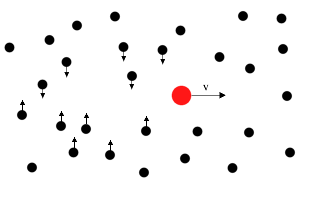
\includegraphics{../kuvat/dynkitka1-v3.png}
\caption*{\hspace{-0.2in}\rule{5in}{0.4pt}}
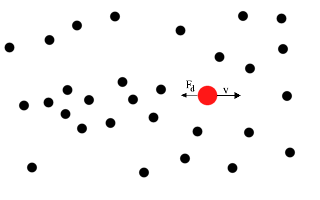
\includegraphics{../kuvat/dynkitka2-v3.png}
\caption{Yksinkertaistettu havainnollistus dynaamisesta kitkasta. Massakappale kulkee hiukkasten seassa, vetäen niitä puoleensa. Nämä hiukkaset liikkuvat massan perään, hidastaen massan kulkua niiden yhteisellä gravitaatiolla. Kuvassa voima $F_d$ kuvaa dynaamista kitkaa.}
\label{fig:dynkitka}
\end{figure}

Mallit kuitenkin paranivat kun otettiin huomioon kaasun hydrodynamiikkaa. Yhdistymisissä kaasu keskittyy keskustaan vuorovesihäiriöiden vuoksi. Tämä kaasu voi luoda nopeaa tähtien syntyä galaksien ohittaessa toisensa ensimmäistä kertaa \citep{mihos:1996}. Tämä sopii hyvin yhteen havaintojen kanssa, sillä galakseilla joissa on voimakasta purskausmaista tähtien syntyä näkyy usein hyvin omituisen muotoisia morfologioita, mikä antaa osviittaa tuoreesta törmäyksestä. Koska monilla kiekkogalakseilla on hyvin paljon kaasua, käy järkeen, että kahden kiekon törmätessä kaasua olisi paljon tarjolla. 

Tämänkaltainen yhdistyminen pystyy simulaatioissa tuottamaan nopeahkosti pyöriviä, kiekkomaisia ellipsejä, mikä vastaa havaittuja keskikirkkaita ellipsejä. Ongelmana kuitenkin on, että tällä tavalla ei oikein saada aikaan hitaasti pyöriviä, laatikkomaisia ellipsejä, jotka vastaavat kaikkein kirkkaimpia havaittuja galakseja. Törmäyksissä mukana oleva dissipatiivinen kaasu aiheuttaa galaksien keskustoihin jyrkkiä huippuja, mikä ei vastaa kirkkaissa ellipseissä havaittuja laakeampia keskusalueita. Lisäksi tämänlaiset hyvin kompaktit ydinalueet myös aktiivisesti haittaavat galaksin tähtien laatikkomaisia ratoja, jotka saisivat aikaan laatikkomaisia isofootteja \citep{gerhard:1985, merritt:1996}.

Simulaatioista on kuitenkin löytynyt mahdollinen ratkaisu tähän ongelmaan. Mikäli tör\-mää\-vissä galakseissa on vähemmän kaasua, kuten jo yhdistymisen seurauksena syntyneissä ellipseissä, törmäyksissä ei ole juuri dissipaatiota ja ne näyttävät synnyttävän ellipsejä, jotka muistuttavat kookkaimpia ja kirkkaimpia havaittuja galakseja. Tuloksena on siis tyyppillisesti hitaasti pyöriviä ja laatikkomaisia ellipsejä \citep{knochfar:2005, naab:2006, cox:2006}. Emogalaksien mustien aukkojen yhdistyminen voisi olla syynä leveämpiin ytimiin.

Kuten kappaleessa \ref{isofootit} alustavasti todettiin, galaksien yhdistyessä dynaaminen kitka saa mustat aukot putoamaan mergerin keskelle. Mustien aukkojen tullessa tarpeeksi lähelle toisiaan ne muodostavat sidotun systeemin ja alkavat kiertää toisiaan binäärinä. Mikäli keskustan tähti päätyy lähelle binääriä, se saa kolmen kappaleen vuorovaituksen (3-body interaction) seurauksena paljon energiaa massiiviselta binäärisysteemiltä, ja päätyy paljon ulommalle radalle keskustasta. Tähti voi saada jopa tarpeeksi energiaa ylittääkseen koko galaksin pakonopeuden. Voimakkaan vuorovaikutuksen kokenut tähti poistuu keskustasta nopeudella $v_\star$, joka on keskimäärin verrannollinen binäärin ratanopeuteen \citep{rantala:2018} :
\begin{equation}
v_\star \sim \mathrm{V_{bin}} = \left( \frac{2 G M_\bullet}{a} \right)^{1/2} \ .
\end{equation}

Tämä prosessi siirtää energiaan mustilta aukoilta ympäröivään tähtipopulaatioon, ja tämän seurauksena mustat aukot lähenevät toisiaan. Energian siirto pystyy levittämään keskustan kompaktin alueen laajemmalle säteelle. Keskimäärin binäärin poisheittämä tähtimassa on kokonaisuutena samaa kokoluokkaa itse binäärin massan kanssa \citep{gualandris:2007}, ja koko tämä prosessi vaikuttaa olevan riittävä yksin selittämään kirkkaiden ellipsien ydinten synnyn \citep{begelman:1980, ebisuzaki:1991, faber:1997, milosavljevic:2002}.

%Kaasua sisältävien galaksien dissipaatiota sisältäviä törmäyksiä sanotaan myös ``märiksi'' törmäyksiksi, kun taas tämänkaltaisia vähemmän kaasua sisältäviä törmäyksiä sanotaan ``kuiviksi''.

Eli vaikka perinteinen, vain kahden kiekkomaisen galaksin yhdistyminen ei pysty tuottamaan kaikenlaisia havaittuja ellipsejä, näyttää siltä, että tällä tavalla usean yhdistymisen ketjuna voi syntyä kaikkia niitä ellipsejä, joita voimme taivaaltakin löytää. Tämä tukee mergereitä pääasiallisena syntytapana ellipsigalakseille. 

\subsection{Baryonisia prosesseja}

%\subsubsection{Fudnamentaalitaso}
Kaavassa \ref{fundamentaalitaso} mainittu fundamentaalitasorelaatio pätee hyvin kaikille ellipseille. Tämän takia on tärkeää katsoa miten törmäyksissä syntyneiden galaksien ominaisuudet vastaavat havaittujen galaksien ominaisuuksia tältä kantilta. Tutkimalla monia eri simulaatioita on havaittu, että toivotunlaisen kallistuneen fundamentaalitason saamiseksi törmäävissä galakseissa täytyy olla kaasua \citep{robertson:2006}. Tämäkin tukee teoriaa, että alunperin ellipsit ovat syntyneet kaasurikkaiden kiekkomaisten galaksien törmäyksissä. 

On havaittu, että punasiirtymillä z $\lesssim$ 1 huomattava osa kirkkaista ellipseistä törmää toisiin ellipseihin \citep{dokkum:2005, bell:2006, mcintosh:2008}. Niinpä onkin tärkeää tutkia, säilyykö fundamentaalitaso tämänlaisissa kaasuköyhissä törmäyksissä. Simulaatiot ovatkin näyttäneet, että sferoidaalisten galaksien väliset törmäykset suunnilleen säilyttävät fundamentaalitason kallistuksen \citep{nipoti:2003, boylan:2005, robertson:2006}.

Empiirisesti on havaittu, että elliptiset galaksit löytyvät lähes yksinomaan isoista galaksijoukoista. Ellipsit muodostuvat siis paikkoihin, joissa on galakseja tiheässä, mikä sopii yhteen teorian kanssa, että ne syntyvät törmäyksistä. Enemmän lähellä olevia galakseja, enemmän galaksien törmäyksiä.

Tutkimalla ellipsigalaksien evoluutiota korkeammilla punasiirtymillä, voimme havaita, että joukoissa sijaitsevat ellipsigalaksit muodostivat suurimman osan tähdistään $z > 2$ \citep{aragon:1993, rakos:1995, ellis:1997, schade:1997, stanford:1998}. Ellipsigalaksien muodostumismallit ennustavat, että massiiviset galaksit muodostuisivat vasta myöhemmin kuin pienemmät, mikä saattaa ensisilmäyksellä sotia sitä vastaan, että isot galaksit sisältävät vanhempia tähtiä. Tämä kuitenkin selittyy sillä, että vaikka massiiviset ellipsit muodostuvat myöhemmin, niiden synnyttäjinä olleet pienemmän massan galaksit syntyivät varhain, ja suurin osa tähtien synnystä olisi siis tapahtunut jo näissä galakseissa.

Yllä on puhuttu kokonaisten galaksien törmäyksistä, mutta merkittävä seikka massiivisten ellipsigalaksien synnyssä on myös pienemmät yhdistymiset. Ellipseihin kertyy tähtiä, jotka ovat muodostuneet itse ellipsin ulkopuolella omissa pienissä alueissaan, jotka ovat syntyneet alkuperäisen törmäyksen aikana. Tämä on merkittävä tekijä ellipsigalaksien kokojen kasvussa punasiirtymältä z $\sim$ 2 nykypäivään asti \citep{naab:2009, johansson:2012}.

Myös galaktiset ulosvirtaukset ovat tärkeä tekijä galaksien muodostuksessa. Galaksien metallit eivät sijoitu vain tähtiensyntyalueille, vaan galakseissa täytyy olla jonkinlaista virtausta joka kuljettaa kuumaa, metallirikasta kaasua muihin galaksin osiin sen syntypaikoilta. Virtaukset myös tekevät galakseista vähemmän tiiviitä ja ne hidastavat tähtienmuodostusta. Tärkeimpiä virtausten lähteitä ovat supernovat, massiivisten tähtien aurinkotuulet ja aktiivisista galaksien ytimimistä syntyvät suihkut \citep{naab:2017}.

%TODO tämä pois? Parannus? Vaatii paljon duunia...
%\subsubsection{Ulosvirtaukset}
%
%Monet simulaatiot ovat osoittaneet, että mikäli galakseissa ei olisi minkäänmoista ulosvirtausta, niistä tulisi aivan liian tiiviitä todellisiin havaintoihin verrattuna. Tämän takia on esitetty erilaisia teorioita ja tapoja sille, mikä hidastaa materian kasautumista galakseissa.
%
%Core-collapse supernovat ovat tärkeässä osassa galaksien muodostumisessa. Tähden räjäh\-täessä tyypillisesti muutaman auringon massan verran kaasua ejektoituu tähtienväliseen aineeseen hyvin suurilla nopeuksilla. Tämä levittää metalleja ympäröivään aineeseen, ja voi kuumentaa läheistä kaasua erittäin kuumaksi. Ne ovatkin päälähde kuumalle ($T \sim 10^6 \, \mathrm{K}$) kaasulle tähtiä muodostavilla alueilla. Nämä räjähdykset ovat iso osa poisvirtausta galakseista, mikä vähentää tähtienmuodostusta. 
%
%Myös massiiviset tähdet vaikuttavat niiden lähialueisiin aurinkotuulten välityksellä. Vaikka ne ovat energeettisesti paljon vähemmän tärkeitä kuin supernovaräjähdykset, aurinkotuulet voivat vähentää ympäröivän kaasun tiheyttä, ja siten lisätä supernovien tehokkuutta. Myös pelkkä tähtien aiheuttama säteilypaine voi vaikuttaa merkittävästi ympäröivään tähtienväliseen aineeseen sekä lämmön että säteilyn aiheuttaman liikemäärän seurauksena. 
%
%Näiden lisäksi tähdistä syntyvät kosmiset säteet ovat ehkä yllättävän tärkeässä roolissa galaktisten virtausten aiheuttajina. Kosmiset säteet jäähtyvät paljon hitaammin kuin terminen kaasu, joten ne voivat kulkeutua pitkiäkin matkoja ja siten vaikuttaa merkittävästi tähtienväliseen aineeseen. 
%
%Tähdistä syntyvien virtausten lisäksi aktiivisista galaksien ytimistä syntyvät suihkut vaikuttavat tähtienväliseen aineeseen sekä kineettisesti että termisesti. 

%\subsection{Himmeimmät ellipsit}
%
%Tähän asti on puhuttu lähinnä kirkkaiden ja keskikirkkaiden ellipsien muodostumisesta. Olisi ehkä luontevaa ajatella, että kääpiöellipsit syntyisivät samalla tavalla kuin niiden isommat kumppanit, mutta pienemmistä galakseista, kuten epäsäännöllisistä galakseista. Tämä kuitenkin ennustaisi, että niitä olisi melko harvassa, kuten epäsäännölliset galaksit. Näin ei kuitenkaan havaintojen mukaan ole, vaan kääpiöellipsit näyttävät olevan yhtä paljon ryppäissä kuin niiden kirkkaammat seuralaiset. Lisäksi kääpiöiden kinematiikka muistuttaa kirkkaita ellipsejä, eli niillä on vain vähän rotaatiota. Kuten yllä on puhuttu, ei ole selvää, miksi kahden kaasurikkaan galaksin törmäyksessä syntyisi hitaasti pyörivä ellipsi. Todennäköistä onkin, että kääpiöiden edeltäjät muuttuvat kääpiöellipseiksi joidenki galaksijoukoille tyypillisten prosessien takia.
%
%Eräs ehdotettu prosessi on, että kääpiöt olisivat syntyneet epäsäännöllisistä galakseista, kun galaksijoukon tähtienvälisen aineen törmäyspaine riipi niiltä iso osan niiden kaasusta. Tämän ei kuitenkaan pitäisi vaikuttaa kovin paljon tähtien kinematiikkaan, joten ei ole selvää, miksi kääpiöt sitten pyörisivät hitaasti. Toinen teoria on, että kääpiöt syntyisivät, kun galaksijoukkojen nopeat ohitukset häiritsevät spiraaligalakseja, muuttaen himmeän spiraalin kääpiöellipsiksi. Vaikka tämä tapa voi lisätä nopeusdispersioita, se ei kuitenkaan näytä pystyvän poistamaan kaikkea rotaatiota. Kolmas teoria on, että galaksijoukon potentiaalin aiheuttamat vuorovesivoimat ovat repineet massiivisempia ellipsejä pienemmiksi. Tämä on ehkä epätodennäköisin teoria, sillä siinä kääpiöillä täytyisi olla samanlaiset metallisuudet kuin massiivisemmilla ellipseillä, mikä ei pidä paikkaansa. Lisäksi keskustan supermassiiviselle mustalle aukolle ei pitäisi käydä mitään, mutta kääpiöissä ei ole havaittu yhtä isoja mustia aukkoja. 
%
%Mitkään edellä mainituista teorioista eivät siis kuitenkaan tällä hetkellä ole aukottomia, ja niissä kaikissa on ongelmansa. Ei siis ole vielä mitään yksittäistä parasta selitystä kääpiiöellipsien muodostumiselle. 

\section{Loppupäätelmät}

Ellipsigalaksit ovat paljon monimuotoisempia systeemeitä kuin voisi aluksi luulla. Kaksi pääluokkaa isoille ellipsigalakseille ovat jättiläismäiset ellipsit ja keskisuuret ellipsit. Kirkkaat jättiläismäiset ellipsit pyörivät hyvin hitaasti, ovat muodoltaan triaksiaalisia, niiden elliptisyys on usein melko pieni, niillä on laatikkomaiset isofootit ja niiden keskustat ovat laakeita. Keskikirkkaat ellipsit pyörivät nopeasti verrattuna kirkkaisiin, niiden muoto on liki litteä pyörähdysellipsoidi, niillä on paljon enemmän vaihtelua elliptisyyksissä kuin kirkkailla ellipseillä, isofootit ovat kiekkomaisia ja keskustat kompakteja ja jyrkkiä.

Tutkimukset ovat osoittaneet, että ellipsit eivät eroa galaktisilta ominaisuuksiltaan liian paljoa spiraaleista. Niitä ympäröi pimeän aineen halot ja niiden keskustoissa lymyää supermassiivisia mustia aukkoja. Monoliittinen romahdus on melko varmasti suljettu pois, ja nykyisin lupaavimmalta näyttävä teoria ellipsigalaksien synnylle ovat mergerit, joko spiraaligalaksien välillä tai sitten kahden ellipsin välillä. Galaksien törmätessä dynaaminen kitka saa galaksit hidastumaan ja uppoamaan yhteen uuden pimeän aineen halon sisään. Keskustan tähtien vuorovaikutukset toisiaan kiertävien mustien aukkojen kanssa muokaa suurten ellipsien keskustoita laakeammiksi. Isojen törmäysten lisäksi myös tähtien kertyminen ellipsien ulko-osiin on isossa roolissa ellipsien kasvuun pienillä punasiitymillä.

\newpage
\clearpage
%Monille galakseille tyypillisiä rakenteita ovat keskuspullistuma, joka koostuu vanhoista tähdistä; litteä kiekko, jossa on kaasua ja nuoria tähtiä; halo, jossa on hyvin vanhoja tähtiä ja pallomaisia tähtijoukkoja; sekä 

% - Kysy näitten sanojen suomennoksia: triaxial, isophote (tasakirkkauskäyrä?, prujuissa pintakirkkauden tasokäyrä, isofootti?), disky (kiekkomainen?), boxy(laatikkomainen?), central cusp, fundamental plane 

%Seuraavat jutut on kirjasta \cite{galaxies}

% - Näyttää simppeleiltä, ei ole
 
% - ei juuri yhtään viileää kaasua, paitsi keskustassa
 
% - monipuolisia, osa pyörii nopeasti, osa ei juuri yhtään
 
% - voi olla esim oblate tai triaxial
 
% -efektiivinen säde $R_e$, sisältää puolet kirkkaudesta. On myös $R_s$, exponential scale length: säde jossa intensiteetti putoaa $e^{-1}$-kertaiseksi
 
% - ominaisuudet komboo, kirkkaat on tod.näk. triaxiaalisia, hitaasti pyöriviä, kun taas himmeemmät on oblateja nopeammin pyöriviä, keskustassa on paljon tähtiä
 
% - kirkkaimmat galaksit on ellipsei, mutta ellipsit on myös yksiä himmeimmistä, yhteistä on vain suurinpiirtein muoto ja se, että ei ole viileää kaasua tai nuoria tähtiä
 
% - voidaan jakaa kolmenlaisiin luokkiin: kirkkaat jättiläismäiset ellipsit, keskikokoiset ellipsit, ja kääpiöellipsit
 
% - kun ellipsistä tiedetään kirkkaus, muut ominaisuudet tulee aikalailla sen mukana
 
% - isophoten isoakselin puolikkaan a ja pikkuakselin puolikkaan b suhde kertoo elliptisyyden kaavalla $\epsilon = 1 - b/a$
 
% - elliptisyys pysyy keskimäärin vakiona, joten galakseja voi luokitella Hubblen tyypisi E$n$, missä $n = 10/\epsilon$
 
% - Hubblen tyyppi riippuu katselusuunnasta

% - ellipsigalaksien valoisuus keskittyy hyvin paljon keskellä, toisin kuin spiraalien diskeissä
 
% - sersichommaa. Voimme käyttää Sérsicin empiiristä kaavaa kuvaamaan galaksin valon jakautumista.
%\begin{equation}
%I(R) = I(R_e) \ \mathrm{exp}\{-b[(R/R_e)^{1/n}]\}
%\end{equation}
% Muuttuja b valitaan siten että $R_e$ on tosiaankin efektiivinen säde. Jos $n>1$, $b \approx 1,999n - 0,327$
% 
% -Jos n = 1, on kyseessä yksinkertainen eksponentiaalinen muoto. Jos n=4, on kyseessä niinsanottu de Vaucouleursin laki, joka kehitettiin vartavasten kuvaamaan ellipsigalaksien valokäyriä
% 
% - keskustan ulkopuolella n=4 kuvaa pintakirkkautta melko hyvin kirkkailla, keskisuurilla ellipseillä. Keskustassa seeing vaikuttaa voimakkaasti siihen kuinka laadukkaita kuvia voimme saada. Satelliitteilla voi saada tarkempia kuvia. Kirkkaimmilla galakseilla keskustojen kirkkaus muuttuu melkolailla vakioksi jollain etäisyydellä. Himmeämmissä keskustan kirkkaus näyttää nousevan niin pitkälle kuin instrumentit pystyvät seuraamaan. Keskikokoisissa 
% 
% - isoimmille ja kirkkaimmille galakseille sopii paremmin muodot joissa n on isompi. kääpiöellipseille n $\approx$ 1 sopii melko hyvin
 
% - toisin kuin spiraaleissa, ellipseissä keskustan kirkkaus on tiiviisti linkittynyt kokonaiskirkkauteen. Kirkkaissa ellipseissa, mitä kirkkaampi galaksi on, sitä matalampi sen keskustan kirkkaus on ja sitä leveämpi sen ydin on.
 
% - himmeimmät ellipsit jakaantuvat kahteen ryhmään: kompakteihin ellipseihin ja kääpioellipseihin ja -sferoidaaleihin. Kompakteilla on huomattavaa pyörimistä, kun taas kääpiöellipsit eivät pyöri merkittävästi. Kääpiösferoidaalit ovat himmeämpiä versioita kääpiöellipseistä. Kaikkein himmeimmissä kohteissa aiemmin mainittu sääntö kirkkaudesta ja keskustasta kääntyy päälaelleen: niissä keskustankin kirkkaus on suhteessa erittäin alhainen. Keskikirkkailla ellipseillä on tyypillisesti kärkipiikki, ei varsinaista ydintä.
% 
% - ellipsigalaksien muoto riippuu katselukulmastamme. Koska näemme galakseja satunnaisista suunista, voimme muodostaa kuvan keskimääräisestä kolmiulotteisesta muodosta käyttämällä hyväksi näennäisten muotojen jakaumaa
% 
% - triaxiaalisissa ellipseissä voi olla isophote twistiä, eli "the position angle of the semimajor axis changes with radius"
% 
% - ellipsigalaksien isofootit eivät yleensä ole täysin elliptisiä. Eroavaisuuksia täydellisestä ellipsistä voidaan kuvata seuraavan funktion Fourier'n kertoimilla
%\begin{equation}
%R_{iso}(\phi)-R_{ell}(\phi) = a_0 + \sum^\infty_{n=1}(a_n \mathrm{cos} (n \phi) + b_n \mathrm{sin} (n \phi)) \ ,
%\end{equation}
% missä $R_{iso}(\phi)$ on isofootin säde kulmalla $\phi$ ja $R_{ell}(\phi)$ on ellipsin säde samalla kulmalla. Yleensä tarkastellaan ellipsiä joka sopii isofoottiin niin hyvin, että kertoimet $a_0, a_1, a_2, b_1$ ja $b_2$ ovat kaikki nolla virherajojen sisällä. Erot tästä parhaan sovituksen isofootista ilmaistaan korkeamman asteen Fourier'n kertoimilla, joilla $n\geq 3$. Erityisen mielenkiintoisia ovat kertoimen $a_4$ arvot, sillä ne kertovat onko isofootti kiekkomainen (disky, $a_4 > 0$) vai laatikkomainen (boxy, $a_4 < 0$). 
% 
% - Toinen tapa kuvata isofootin eroja täydellisestä ellipsistä on määrittää kuinka paljon intensiteetti vaihtelee parhaan sovituksen ellipsillä:
%\begin{equation}
%I(\phi) = I_0 + \sum^\infty_{n=1}(A_n \mathrm{cos} (n \phi) + B_n \mathrm{sin} (n \phi)) \ ,
%\end{equation}
%missä $I_0$ on parhaan sovituksen ellipsin intensiteetti. Kertoimet $A_n$ ja $B_n$ liittyvät suurinpiirtein kertoimiin $a_n$ ja $b_n$ seuraavasti:
%\begin{equation}
%A_n = a_n \left| \frac{\mathrm{d}I}{\mathrm{d}R} \right|, \ B_n = b_n \left| \frac{\mathrm{d}I}{\mathrm{d}R} \right| \ ,
%\end{equation}
%missä $R=a \sqrt{1-\varepsilon}$, jossa $\varepsilon$ on parhaan sovituksen ellipsin elliptisyys.
%
% - disky tai boxy erotus on tärkeä, sillä niissä on systemaattisia eroja
% 
% - boxyissä enemmän isophote twistiä, koska ne ovat useimmiten kirkkaita ja siten todennäköisemmin triaxiaalisia. Pyörivät hitaasti ja niissä on keskivertoa voimakkaampia radio- ja röntgenemissiotia.
% 
% -diskyt ovat himmeämpiä, niissä on merkittävää pyörimistä, ja vähän tai ei ollenkaan radio- tai röntgenemissioita. Nämä ovat yleensä keskikokoisia. Diskiness myös korreloi ytimen ominaisuuksien kanssa: diskyillä ellipseillä on tyypillisesti jyrkät huiput/cuspit, kun taas boxyillä on enimmäkseen central coreja
 
% -6.2 tähtihommaa
 
% - Toisin kuin spiraaligakaseissa, ellipsigalaksien tähtien rotaatio ei seuraa säännönmukaista kaavaa, vaan suurin osa niiden kineettisestä energiasta on satunnaisliikkeessä. Ja kuten spiraaligalaksien kirkkaus on yhteydessä niiden pyörimiseen, kirkkailla ellipsigalakseilla on suurempia nopeusdispersioita kuin himmeämmillä. Tämän yhteyden avulla voimme määrittää etäisyyksiä galakseihin. Ellipsigalaksit pyörivät yllättävän hitaasti, mikä osoittaa, että tähdet eivät ole vielä relaksoituneet mihinkään lopulliseen tilaan, vaan niiden alkuperästä on vielä paljon pääteltävissä.
% 
% -Galakseissa olevien tähtien ratanopeuksien määrittäminen on hankalaa, sillä toisin kuin kaasupilvissä, joissa voimme melko helposti katsoa emissioviivoja, tähdissä meidän täytyy katsoa absorptioviivoja. Nämä eivät yleensä ole siistejä ja kapeita atomiviivoja, vaan ne ovat itsessään leveitä. Viivan keskustan sijainnin lisäksi meidän täytyy huomioida myös viivan leveys ja muoto. Tämä vaatii korkeaa signaali-kohinasuhdetta ja pitkiä havaintoaikoja.
% 
% - Kaikkien galaksin tähtien valo on summa niiden yksittäisistä spektreistä. Jokainen spektri on Doppler-siirtynyt oman liikkensä mukaisesti, ja näiden rataliikkeiden takia tähtien yhteinen spektri on leveämpi ja matalampi kuin yksittäisten tähtien. Ellipsigalakseissa ei ole paljoa viileää kaasua, joten galaksin valo vastaa aika lailla tähtien emittoimaa valoa.
% 
% - Ellipsigalakseilla on faber-jackson:1976 relaatio, joka antaa karkean arvion kirkkauden ja nopeusdispersion yhteydelle: $L \propto \sigma^4$. Voimme verrata tästä relaatiosta saatua todellisen kirkkauden arviota havaittuun kirkkauteen, ja saada siten arvion galaksin etäisyydelle. Galaksista tulleen valon kokonaismäärää on kuitenkin hankala määrittää, sillä iso osa siitä tulee galaksin himmeistä ulko-osista. Tämän takia faber-jackson:1976 relaatiosta saadut arvot ovat melko suuntaa antavia. Tarkempi tapa on mitata halkaisija galaksin alueesta, jossa pintakirkkaus on keskiarvoltaan valitun suuruinen. Tiedämme että keskuskirkkaus riippuu kokonaiskirkkaudesta, joten voimme muodostaa yhteyden nopeusdispersion ja halkaisijan välille. Tästä voimme saada etäisyysarvion kun tiedämme kuinka isolta galaksi näyttää Maasta katsottuna.
 
% - selitystä ellipsien pyörimisestä ja sen hitaudesta?
% 
% - seuraavaks 6.3
 
% - Toisin kuin epäsäännöllisissä galakseissa ja spiraaligalakseissa, ellipseissä ei näy kirkkaita sinisiä tähtiä. Kirkkaimpia tähtiä näissä galakseissa ovat sen sijaan asymptoottihaaran tähdet. Vain vähän valosta on aallonpituudeltaan alle 3500 Ångströmiä, mikä osoittaa että ellipsigalakseissa on syntynyt erittäin vähän tähtiä viimeisen parin miljardin vuoden aikana. Toisaalta vain tähdet joiden massa on alle 2 $M_\odot$ elävät yli miljardi vuotta, ja nämä tuottavat isoimman osan valostaan jättiläisvaiheessa. Joten ellipsigalaksien valo on pääosin peräisin punaisista jättiläisistä. Kuten aiemmin todettiin, ellipsigalaksien muut ominaisuudet ovat yhteydessä kirkkauteen. Samaten galaksin väri ja kirkkaus ovat linkittyneitä näkyvän valon alueella ja lähi-infrapunassa. Kirkkaammat galaksit ovat punaisempia ja himmeämmät sinisempiä. 
 
% - juttua siitä miksi väriyhteys on olemassa, monia eri selityksiä. Kaasua ellipseissä
 
% - Katsomalla ellipsigalaksien massa-valo-suhteita ja pyörimisnopeuksia kaukana keskustasta, voimme päätellä, että myös ellipsigalakseissa täytyy olla pimeää ainetta, kuten spiraaligalakseissakin. Voimme havaita mustia aukkoja epäsuorasti katsomalla keskustassa olevien tähtien liikkeitä. Mikäli keskustan tähtien nopeusdispersio on paljon suurempi kuin muualla ympärillä, voimme päätellä että keskellä täytyy olla jokin hyvin massiivinen kohde. Havainnot ellipsigalakseista näyttävät että näin todellakin on myös ellipsigalakseissa, mikä antaisi olettaa että myös niissä on keskustassa massiivinen musta aukko. Isoimmat keskusmassat on löydetty galakseista joissa on isoimmat nopeusdispersiot.


%Nämä jutut on pääosin \cite{galform}
%
% - kirkkailla ellipseillä litteys johtuu nopeus anisotropiasta, ei pelkästä pyörimisestä
 
% - nopeusdispersio nousee voimakkaasti keskuksissa, ja tämän on yleisesti käsitetty johtuvan siitä, että keskustasa on musta aukko, joka vaikuttaa voimakkaasti keskustan havaittaviin tähtiin
 
% -ellipsit joilla on korkea (keskustan) nopeusdispersio ovat kirkkaampia (faber-jackson:1976) ja isompia (D-$\sigma$ relaatio)
 
% - ellipseissä on paljon tähtienvälistä ainetta, mutta sillä on hyvin erilaiset ominaisuudet kuin spiraaligalakseissa
% 
% - Kuuma ($\sim 10^7$ K), röntgensäteitä emittoiva kaasu muodostaa suurimman osan tähtienvälistä ainetta, jopa $\sim 10^{10} M_\odot$. Tämän lisäksi useimmissa ellipsigalakseissa on lämmintä ($10^4$ K) ionisoitunutta kaasua ja kylmää ($<100$ K) kaasua ja pölyä. Tyypillisiä massoja on $10^2 - 10^4 M_\odot$ lämpimälle kaasulle ja $10^6 - 10^8 M_\odot$ kylmälle aineelle. Toisin kuin spiraaleissa, pölyn ja kaasun määrät eivät korreloi kirkkauteen. 
 
% - Kinematiikan ja fotometrian perusteella ellipsit voi jakaa karkeasti kolmeen luokkaan. Kirkkaille ellipseille ($M_B \lesssim -20,5$) tyypillistä ovat vähäinen pyöriminen, boxyt isophotet, pieni elliptisyys ($\varepsilon \lesssim 0,3$), ja suhteellisen loivat keskustan kirkkausprofiilit. Keskikirkkailla ellipseillä ($-20,5 \lesssim M_B \lesssim -18$) puolestaan pyöriminen tukee niiden rakennetta merkittävästi, niillä on diskyjä isophoteja, elliptisyys vaihtelee enemmän ($\varepsilon \lesssim 0,7$), ja keskustan kirkkausprofiileissa on jyrkkiä cuspeja. Himmeämmässä päässä ($M_B \gtrsim -18$) on kääpiöellipsejä ja kääpiösferoidaaleja. Niillä ei näytä olevan juurikaan pyörimistä ja niiden kirkkauskäyrät ovat kutakuinkin eksponentiaalisia. 
 
% - Diskiness tulktiaan usein seuraukseksi  ellipsigalaksissa olevasta kiekkorakenteesta (lisää selitystä pls)
% 
% - Diskyt ellipsit näyttävät siis muodostavan jatkuvan sarjan (onko tyhmästi sanottu?) S0 galakseista varhaisemman tyypin galakseihin.
 
% - Isolla osalla boxyistä ellipseistä on isophote twistingiä. Tämä on mahdotonta akselisymmetrisille systeemeille, mutta tapahtuu luontaisesti jos galaksi on triaxiaalinen.Tämän takia kirkkaiden ellipsien usein ajatellaan olevan triaxiaalisia. Diskyillä taas ei puolestaan näy isophote twistingiä juuri koskaan, mikä sopii yhteen käsityksen kanssa että ne ovat akselisymmetrisiä.
 
% - vaikka isolla osalla pienistä ellipseistä ei ole juuri pyörimistä, noin 20\%:lla niiden kinematiikka näyttää siltä, että pyöriminen aiheuttaa niiden littoisuuden.
% 
% - diskyt ellipsit ovat todennäköisesti kahden komponentin systeemejä (kiekko ja ellipsi), vähän kuten S0:t.
% 
% jatkuu pedari sivu 599
 
% - kinematic misalignment, jotain siitä ehkä
 
% - Litteälle pyörähdysellipsoidille kinemaattinen akseli, eli akseli jonka suuntaisesti havaittu pyörimisnopeus on nolla, osuu yhteen fotometrian pikkuaskelin kanssa. Osalla ellipseistä on kuitenkin havaittu olevan rotaatiota sekä iso- että pikkuakselin suhteen. Niiden kinemaattiset ja fotometriset akselit eivät siis täsmää. Tälläinen kinemaattinen epäkohdistus(???) on yleisempää kirkkaammissa ellipseissä joita tukee nopeusdispersio. Nopeasti pyörivissä ellipseissä sitä ei juuri havaita. 
% 
% - Noin neljänneksellä ellipseistä on kinemaattisesti irtikytkeytynyt ydin (kinematically decoupled core (KDC)), jonka kulmaliikemäärävektori ei osu yksiin koko galaksin kanssa. Äärimmäisissä tapauksissa keskusta voi jopa pyöriä eri suuntaan kuin muu galaksi. Tällaiset ytimet on yleensä selitetty dynaamisesti erillisinä alijärjestelminä, jotka ovat jäämiä yhdistyneistä kumppaneista. Vaihtoehtoinen syy tällaiselle kinemaattiselle vääntymiselle voi löytyä ympyräratojen projisoitumisesta triaxiaalisessa potentiaalissa (mitä tää oikeestaan meinaa?). Tämäntyyppisten ellipsien fotometria tai nopeusdispersioprofiilit eivät eroa merkittävästi tavallisesta, joten ei ole täysin selvää mikä on oikea syy tähän ilmiöön.
 
% - Spiraaligalakseissa neutraalin vedyn rotaatiokäyrät ovat vahva todiste pimeän aineen olemassaololle. Ellipsigalakseissa pimeän aineen tutkiminen on kuitenkin haastavampaa, sillä niissä ei ole yhtä hyviä ja helposti tulkittavia indikaattoreita isoilla säteillä. Yksi keino on käyttää hyväksi tähtien kinematiikkaa, jota saadaan integroidun valon absorptioskeptroskopiasta. Tämä keino kuitenkin toimii hyvin vain noin yhden efektiivisen säteen päähän, sillä ellipsien pintakirkkaus tippuu nopeasti säteen kasvaessa. Tällä tavalla mitatut kinematiikat ovat näyttäneet, että tyypillisesti näkösäteen suuntainen %TODO kai line-of-sight on näkösäteen suuntainen?
%nopeusdispersioprofiili on kutakuinkin vakio yhdestä efektiivisestä säteestä ulospäin. Tämä vastaa massa-valo-suhdeprofiilia %TODO oikeenkirjotus
%joka kasvaa ulospäin, jollainen on odotettavissa mikäli systeemin ympärillä on pimeän aineen halo. Säteen suhteen vakiona pysyvä nopeusdispersio voi toisaalta olla myös merkki siitä, että nopeusdispersio muuttuu enemmän tangentiaalisesti anisotrooppiseksi säteen kasvaessa.
%
%
% - Ellipsigalaksien keskusalueiden massa-valo-suhteiden perusteella voidaan sanoa, että yhden efektiivisen säteen sisällä keskimäärin  30\% massasta on pimeää ainetta.
% 
% - Toinen tapa massajakumien tutkimiseen suurillä säteillä on käyttää hyväksi diskreettejä dynaamisia tracereitä, kuten pallomaisia tähtijoukkoja, planetaarisia sumuja tai satelliittigalakseja. Tracereitä voi seurata suurillekin säteille, mutta niiden säteittäisnopeuksien dynaaminen mallintaminen kärsii samasta massa-anisotropiasta kuin integroitujen valomittausten tulkitseminen. Lisäksi sopivia tracereitä on melko harvassa, joten tarkkojen tulosten saaminen on haastavaa.
% 
% - Dynaamisen mallintamisen lisäksi ellipsigalaksien potentiaaleja voi tutkailla röntgenkartoituksen ja gravitaatiolinssien avulla.
 
% Seuraavaks s. 603 13.1.6 mustat aukot
 
% - Mustia aukkoja on etsitty paljon läheisistä galakseista kinemaattisten tutkimusten avulla. Erityisesti yritetään löytää näyttöä massa-valo-suhteen kasvusta galaksien keskustassa mitä ei voida selittää tavallisilla tähtipopulaatioilla. Tämä voi osoittaa supermassiivisen mustan aukon olemassaolosta, mutta se voi johtua myös isosta määrästä himmeitä kohteita, kuten ruskeita kääpiöitä tai tähtien jäänteitä. Kuitenkin jos havaittu massa-valo-suhde on tarpeeksi iso ja rajoittuu tarpeeksi pienelle alueelle, voidaan nämä muut vaihtoehdot rajata pois sillä perusteella, että niillä olisi paljon galaksin ikää pienemmät eliniät.
% 
% - Kuten aiemmmin mainittiin, monilla ellipsigalakseilla on nopeusdispersioprofiilit jotka nousevat jyrkästi keskustaa kohti. Yksinkertaisten isotrooppisten mallien sovittaminen osoittaa massa-valo-suhteen kasvua keskustassa, mikä sopii yhteen supermassiivisen mustan aukon olemassaolon kanssa. Tämä ei ole kuitenkaan yksiselitteistä, sillä sama massa-anisotropia joka on ongelmana halojen tutkimisessa haittaa myös tätä työtä. Keskustan nopeusdispersio voi olla suuri myös systeemissä jossa ei ole suurta mustaa aukkoa jos keskusta on säteittäisesti anisotrooppinen. Tämä epäselvyys voidaan kuitenkan melko hyvin poistaa mittaamalla koko näkösäteensuuntaisen nopeusdispersio. Tämä tarkempi data, yhdistettynä kehittyneisiin malleihin, ovat antaneet vahvaa näyttöä supermassiivisille mustille aukoille muutamassa tusinassa läheisessä ellipsigalaksissa.
% 
% - Nykyään yleisesti hyväksytty, että jokaisessa suhteellisen massiivisessa galaksissa on supermassiivinen musta aukko sen keskellä. 
 
% - litistyminen voi johtua rotaatiosta tai sitten anisotrooppisesta nopeusdispersiosta
% 
% 13.2., kato tätä lisää evoluutioteoriakappaleisiin
 
% - Ellipsigalaksien dynaaminen rakenne on paljon vähemmän järjestäytynyt kuin kiekkomaisten galaksien, mikä antaa viitteitä siitä, että niiden muodostuminen oli paljon rajumpaa. Kaikki ellipsigalaksien muodostumisteoriat olettavatkin, että voimakkaalla relaksaatiolla (jossa siis potentiaali vaihtelee hyvin paljon) oli tärkeä osa jossain vaiheessa muodostumisprosessia. On havaittu, että voimakas relaksaatio joko kylmän ja epäsymmetrisen alkutilan romahtamisen aikana tai kahden suunnilleen samanmassaisen kohteen yhdistymisen jälkeen tuottaa  ellipsoidimaisia systeemejä, joiden tiheysprofiilit täsmäävät ellipsigalakseja. 
 
% - dissipationless or 'dry' merger: no gas, \\
% dissipative or 'wet' merger: has gas
 
% - kato lisää galform lecture 12 
 
% 13.4.
% 
% - fundamental plane
 
% - Ellipsigalakseilla on tiukka yhteys keskustan nopeusdispersion, efektiivisen säteen ja efektiivisen säteen sisäisen pintakirkkauden välillä. Tämä on niin sanottu fundamentaalitaso (fundamental plane). Se on yleisesti määritelty kaavalla
% 
%\begin{equation}
% \mathrm{log} \, R_e = a \, \mathrm{log} \, \sigma_0 + b \, \mathrm{log} \, \langle I \rangle_e + \mathrm{vakio}.
%\end{equation}
%
%Tyypillisesti parhaan sovituksen parametrit ovat välillä $a \sim 1,2$ (sininen) ja $a \sim 1,5$ (lähi-infrapuna), ja $b \simeq -0,8$ (ei juuri riippuvuutta fotometrisestä kaistasta).
 
% -dissipationless kiekkomergerit tuottavat viriaalirelaation ehdottamia vakion arvoja, kun taas kaasua sisältävien galaksien mergerit tuottavat tilttiä, kuten on havaittu
 
% - Ennen kuin fundamentaalirelaatio havaittiin, Faber \& Jackson huomasivat, että ellipsigalaksin luminositeetti korreloi sen keskustan nopeusdispersion kanssa kutakuinkin $L \propto \sigma^4_0$. Tämä faber-jackson:1976-relaatio on samanlainen kuin Tully-Fisher-relaatio spiraaligalakseille. Koska $L \propto \langle I \rangle_e R^2_e$, faber-jackson:1976-relaatio implikoi FP relaatiota jossa $a = 2$ a $b = -1/2$. Nämä arvot ovat melko erilaisia havaitun FP relaation parhaista sovituksista, mikä osoittaa, että faber-jackson:1976-relaatio on kaukana FP:n edge-on projektiosta 
 
% 13.5. tähtipopulaatiot
 
% - Tähtipopulaatiota karakterisoi sen tähtienmuodostushistoria (star-formation history, SFH), lähtömassafunktio (initial mass function, IMF), sekä kemiallisen rikastumisen historia. 
% 
% - Varhaisen tyypin galakseille on havaittu väri-magnitudi-korrelaatio, eli niiden niiden väri korreloi vahvasti luminositeetin kanssa. Tämän perusteella ei voi kuitenkaan suoraan todeta mitään tähtipopulaation fysikaalisista ominaisuuksista, sillä ikä-metallisuus-degeneraatio haittaa tätä. Nuoret tähdet joilla on korkea metallisuus näyttävät samanlaisilta kuin vanhat tähdet joilla on vain vähän metalleja. Nykyään useat tutkimukset ovat samaa mieltä siitä, että relaatio värin ja magnitudin välillä johtuu pääosin metallisuudesta, ei iästä.
% 
% - Absorptioviivat antavat paremman kuvan tähtipopulaatioista, sillä niiden avulla päästään eroon edellä mainitusta degeneraatiosta. On havaittu, että osa viivoista ovat herkempiä iälle, kun taas osasta näkee paremmin populaation metallisuuden. Ellipsigalaksien tähtien iät näyttävät olevan laajalla välillä, noin kahdesta gigavuodesta aina universumin alkuajoille asti. Metallisuudet puolestaan näyttävät olevan aika pienellä välillä. 
 
% - Myös tutkimalla ellipsigalaksien evoluutiota korkeammilla punasiirtymillä voimme havaita, että joukoissa sijaitsevat ellipsigalaksit muodostivat suurimman osan tähdistään $z > 2$, ja ne ovat kehittyneet passivisesti sen jälkeen.
% 
% - Ellipsigalaksien muodostumismallit ennustivat, että massiiviset galaksit muodostuisivat myöhemmin, mikä ei sopisi yhteen datan kanssa, että isot galaksit sisältävät vanhempia tähtiä. Tämä voi kuitenkin selittyyä sillä, että vaikka massiiviset ellipsit muodostuvat myöhemmin, niiden synnyttäjinä olleet massiiviset galaksit syntyivät varhain. 

% - Kirkkaita ellipsiejä ja kääpiöellipsejä tukevat lähinnä anisotrooppiset nopeusdispersiot, kun taas keskikirkkaat galaksit ovat pyörimisen takia litistyneitä. 
% 
% 13.6.
 
% - Kääpiöellipsit eivät näytä olevan peräisin samasta syntymekanimsista kuin niiden isommat kumppanit. Sen sijaan niitä löytyy lähinnä isoista galaksijoukoista, joten on luultavaa, että ne ovat jäännöksiä edeltäneistä galakseista, jotka ovat muuttuneet joidenkin joukolle ominaisten prosessien takia. Ei kuitenkaan ole vielä mitään yksittäistä parasta selitystä näiden kääpiöiden muodostumiselle. 
 
 %pupen prujut
% galkos prujut
 
% - Ellipsigalaksit löytyvät lähes yksinomaan isoista galaksijoukoista joissa on suuri tiheys. Tämä sopii yhteen teorian kanssa, että ne muodostuivat galaksien yhteentormayksissä. 
 
% - Viriaaliteoreema: miten *keskimäärin* kineettinen ja potentiaali-energia ovat tasapainossa.
% 
% - Mikäli tähtijoukko tai galaksi ovat tasapainossa, voimme laskea viriaaliteoreemalla arvion massalle. 
 
% - mainitse dynaaminen kitka kun puhutaan ellipsien muodostumisesta
 
% - relaksaatio: kappaleet saavat gravitaatiosta "potkuja" liikkuessaan, ajan saatossa niiden radat muuttuvat niin, ettei alkuperäisestä radasta voi sanoa mitään
 
% - Tähtien liike ellipseissä: Ellipsigalakseissa ei ole yleisesti järjestäytynyttä liikettä. Ellipsit ovat tyypillisesti triaksiaalisia ja potentiaalit ovat ei-aksisymmetrisiä. Tähtien radat voidaan jakaa pääsääntöisesti 'loop'-ratoihin, joilla on jokin pyörimissuunta, sekä 'box'-ratoihin, jotka kulkevat galaksin keskustan läpi. 
 
% - Galaksien relaksaatioajat ovat hyvin pitkiä, joten tähtien radoista voi tehdä päätelmiä niiden syntymekanismeista. 
 
% - Epäsymmetriat pinkakirkkauksissa antavat vihiä siitä, että ne ovat olleet osallisia galaksien törmäyksissä.
 
% - Ellipsit voidaan jakaa ytimen pintakirkkauden perusteella core-ellipseihin ja cusp-ellipseihin. Core-ellipseissä ytimen pintakirkkaus on melkein vakio, eli niiden keskustasta "puuttuu valoa". Nämä galaksit ovat tyypillisesti isoja ja niiden keskustassa on massiivinen musta aukko. Cusp-ellipseissä puolestaan ytimen pintakirkkaus on hyvin suuri, eli niiden keskustassa on "liikaa valoa". Nämä ovat yleensä pienimassaisempia ja pyörivät core-ellipsejä nopeammin.
 
% - Triaksiaalisessa galaksissa on kolme riippumatonta akselia, a, b, c, joiden ympäri tähdet voivat liikkua. 
 
% - Ellipseissa isofoottien litistyneisyys voi muuttua säteen funktiona (isophote twist). Tässä tapauksessa ei voi kyseessä olla puhdas pyörähdysellipsoidi, vaan sen täytyy olla triaksiaalinen. 
 
% - Ellipsigalaksien valoa dominoi K- ja M-tyypin punaiset jättiläiset, minkä ansiosta näillä galakseilla on hyvin vahvat absorptioviivat. Nuoria massivisia sinisiä tähtiä ei ole käytännössä juuri ollenkaan. 
 
% - Ellipsigalakseissa on tyypillisesti erittäin vähän kylmää kaasua, vain luokkaa $10^8 - 10^9 M_\odot$, minkä takia uusien tähtien muodostusta ei juuri ole. Kuumaa inisoitunutta kaasua puolestaan on enemmän ($10^9 - 10^{11} M_\odot$). Tämä kaasu on peräisin jättiläistähtien ulko-osista.
 
% - Radiogalaksit aina ellipsejä
 
% - Dynaaminen kitka galakseissa on verrannollinen toisen galaksin massatiheyteen
% 
% - Galaksien ohituksessa osa liike-energiasta siirtyy tähtien satunnaisliikkeeseen. 
% 
% - Dynaaminen kitka on tehokkaampaa hitaammilla kohteilla
% 
% - Dynaaminen kitka siirtää kiertävilta galakseilta ja pimeän aineen haloilta rataenergiaa host halon pimeän aineen kappaleisiin, mikä saa kiertolaisen "uppoamaan" potentiaalinkuopan keskelle, missä se voi lopulta yhdistyä toiseen galaksiin.
 
 

%%%%% Sisältö loppuu, lähdeluettelo %%%%%
\addcontentsline{toc}{section}{Viitteet}
\bibliographystyle{plainnat}
\small
\bibliography{lahteet}

%\appendix
%%\newpage
%\section{Tärkeä liite}
%Lorem ipsum.
%\newpage



\end{document}
